\documentclass[xcolor=dvipsnames]{beamer}
\usepackage[T1]{fontenc}
\usepackage[utf8]{inputenc}
\usepackage[english,slovak]{babel}

\usepackage{amsmath}
\usepackage{amsthm}
\usetheme{Pittsburgh}
\useoutertheme{shadow}

\usepackage{graphicx}
\usepackage{caption}
\usepackage{subcaption}

\usepackage[]{algorithm2e}
\usepackage{listings}
 \setbeamercovered{transparent}
 \usepackage{cuted}
\usepackage[export]{adjustbox}
\usepackage{mathtools}

\usepackage{lipsum}
\usepackage{verbatim}
\usepackage{transparent}
\usepackage{framed}
\usepackage{xcolor}

\usepackage{multirow}
\usepackage{colortbl}
\usepackage{lmodern}

\usepackage{movie15}
\usepackage{media9}
\usepackage{verbatim}

\usepackage{animate}


\usepackage{hyperref}

\newcommand\Wider[2][3em]{%
\makebox[\linewidth][c]{%
  \begin{minipage}{\dimexpr\textwidth+#1\relax}
  \raggedright#2
  \end{minipage}%
  }%
}






\iftrue

\usetheme{Warsaw}

\setbeamercolor{normal text}{fg=white,bg=black!90}
\setbeamercolor{structure}{fg=white}

\setbeamercolor{alerted text}{fg=red!85!black}

\setbeamercolor{item projected}{use=item,fg=black,bg=item.fg!35}

\setbeamercolor*{palette primary}{use=structure,fg=structure.fg}
\setbeamercolor*{palette secondary}{use=structure,fg=structure.fg!95!black}
\setbeamercolor*{palette tertiary}{use=structure,fg=structure.fg!90!black}
\setbeamercolor*{palette quaternary}{use=structure,fg=structure.fg!95!black,bg=black!80}

\setbeamercolor*{framesubtitle}{fg=white}

\setbeamercolor*{block title}{parent=structure,bg=black!60}
\setbeamercolor*{block body}{fg=black,bg=black!10}
\setbeamercolor*{block title alerted}{parent=alerted text,bg=black!15}
\setbeamercolor*{block title example}{parent=example text,bg=black!15}

\fi



%-------------------------------------------------------------------------------------
\title{\color{white} \bf deep reinforcement learning - introduction}
\author{\color{white} Michal CHOVANEC, PhD}


%\setbeamertemplate{footline}[frame number]{}
\setbeamertemplate{navigation symbols}{}


\date[EURP]{}
\begin{document}

{
    \usebackgroundtemplate
    {
        \vbox to \paperheight{\vfil\hbox to \paperwidth{\hfil

        {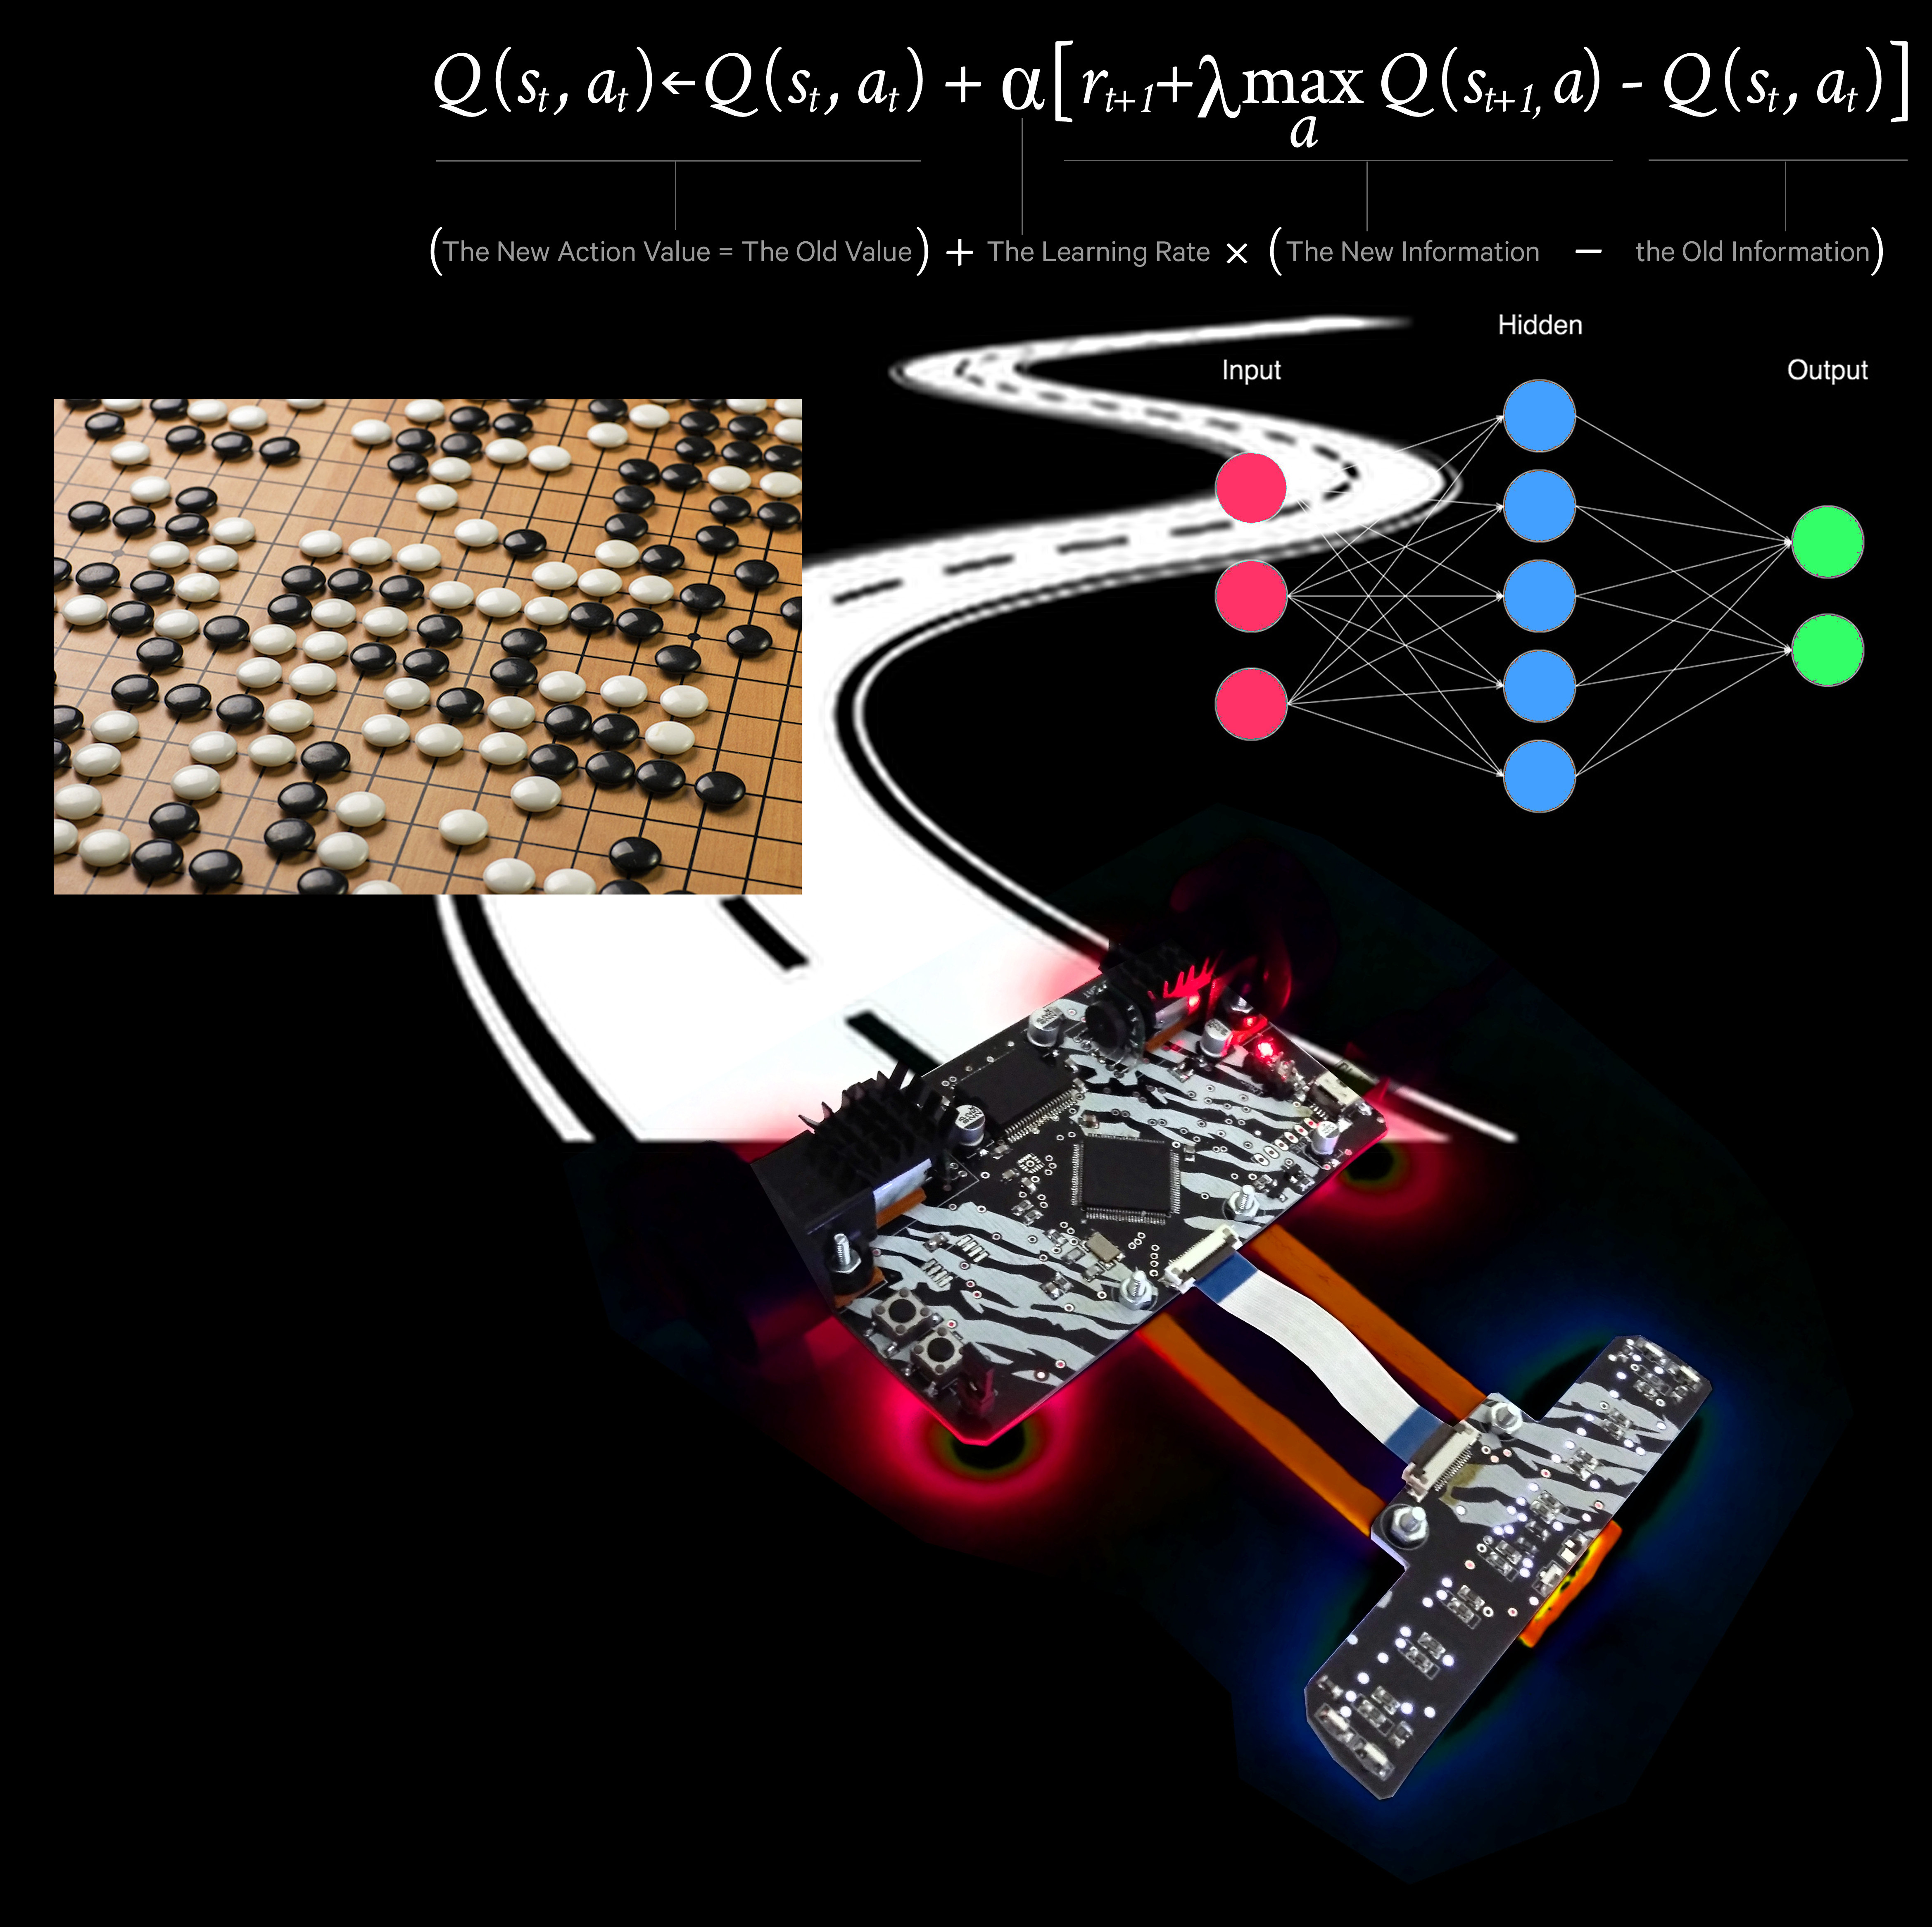
\includegraphics[width=5.05in]{../images/rl_square.jpg}}

        \hfil}\vfil}
    }



    \begin{frame}

    \centering
     \colorbox{black}
     {
        \begin{minipage}{8cm}
           {\LARGE \color{white}deep reinforcement learning} \\
           {\Large \color{white}- introduction} \\
           {\LARGE \color{white} Michal CHOVANEC} \\
       \end{minipage}
     }

    \end{frame}
}


\begin{frame}{\bf deep reinforcement learning - playing Atari}

  \begin{columns}

    \begin{column}{0.5\textwidth}
      \centering{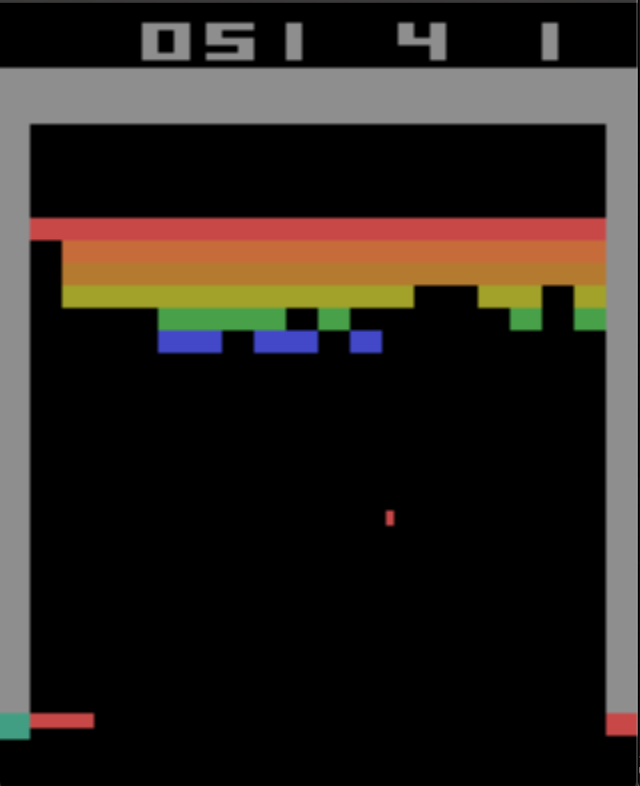
\includegraphics[scale=0.35]{../images/breakout.png}}
    \end{column}

    \begin{column}{0.5\textwidth}
      \centering{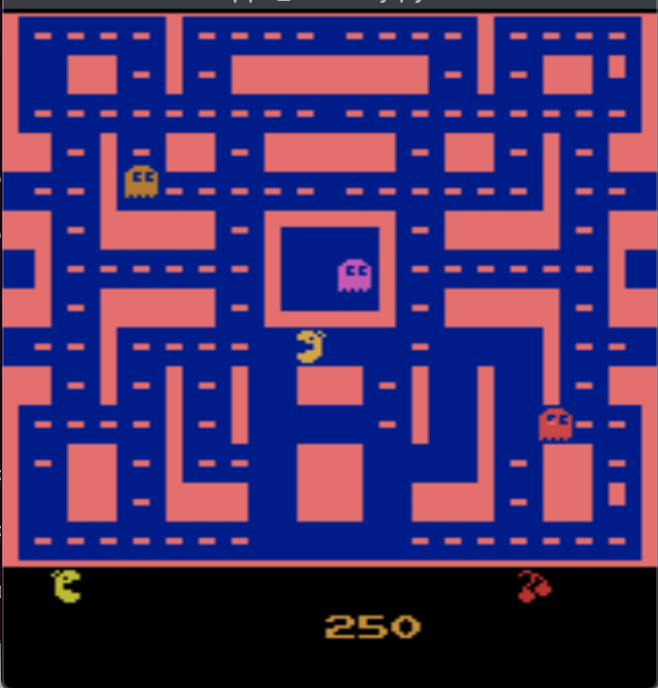
\includegraphics[scale=0.3]{../images/pacman.png}}
    \end{column}

  \end{columns}

  2013, Mnih (DeepMind) : Playing Atari with Deep Reinforcement Learning, 
  \url{https://arxiv.org/pdf/1312.5602.pdf}
\end{frame}


\begin{frame}{\bf reinforcement learning - path to superhuman score}

  \begin{columns}

    \begin{column}{0.5\textwidth}
      \centering{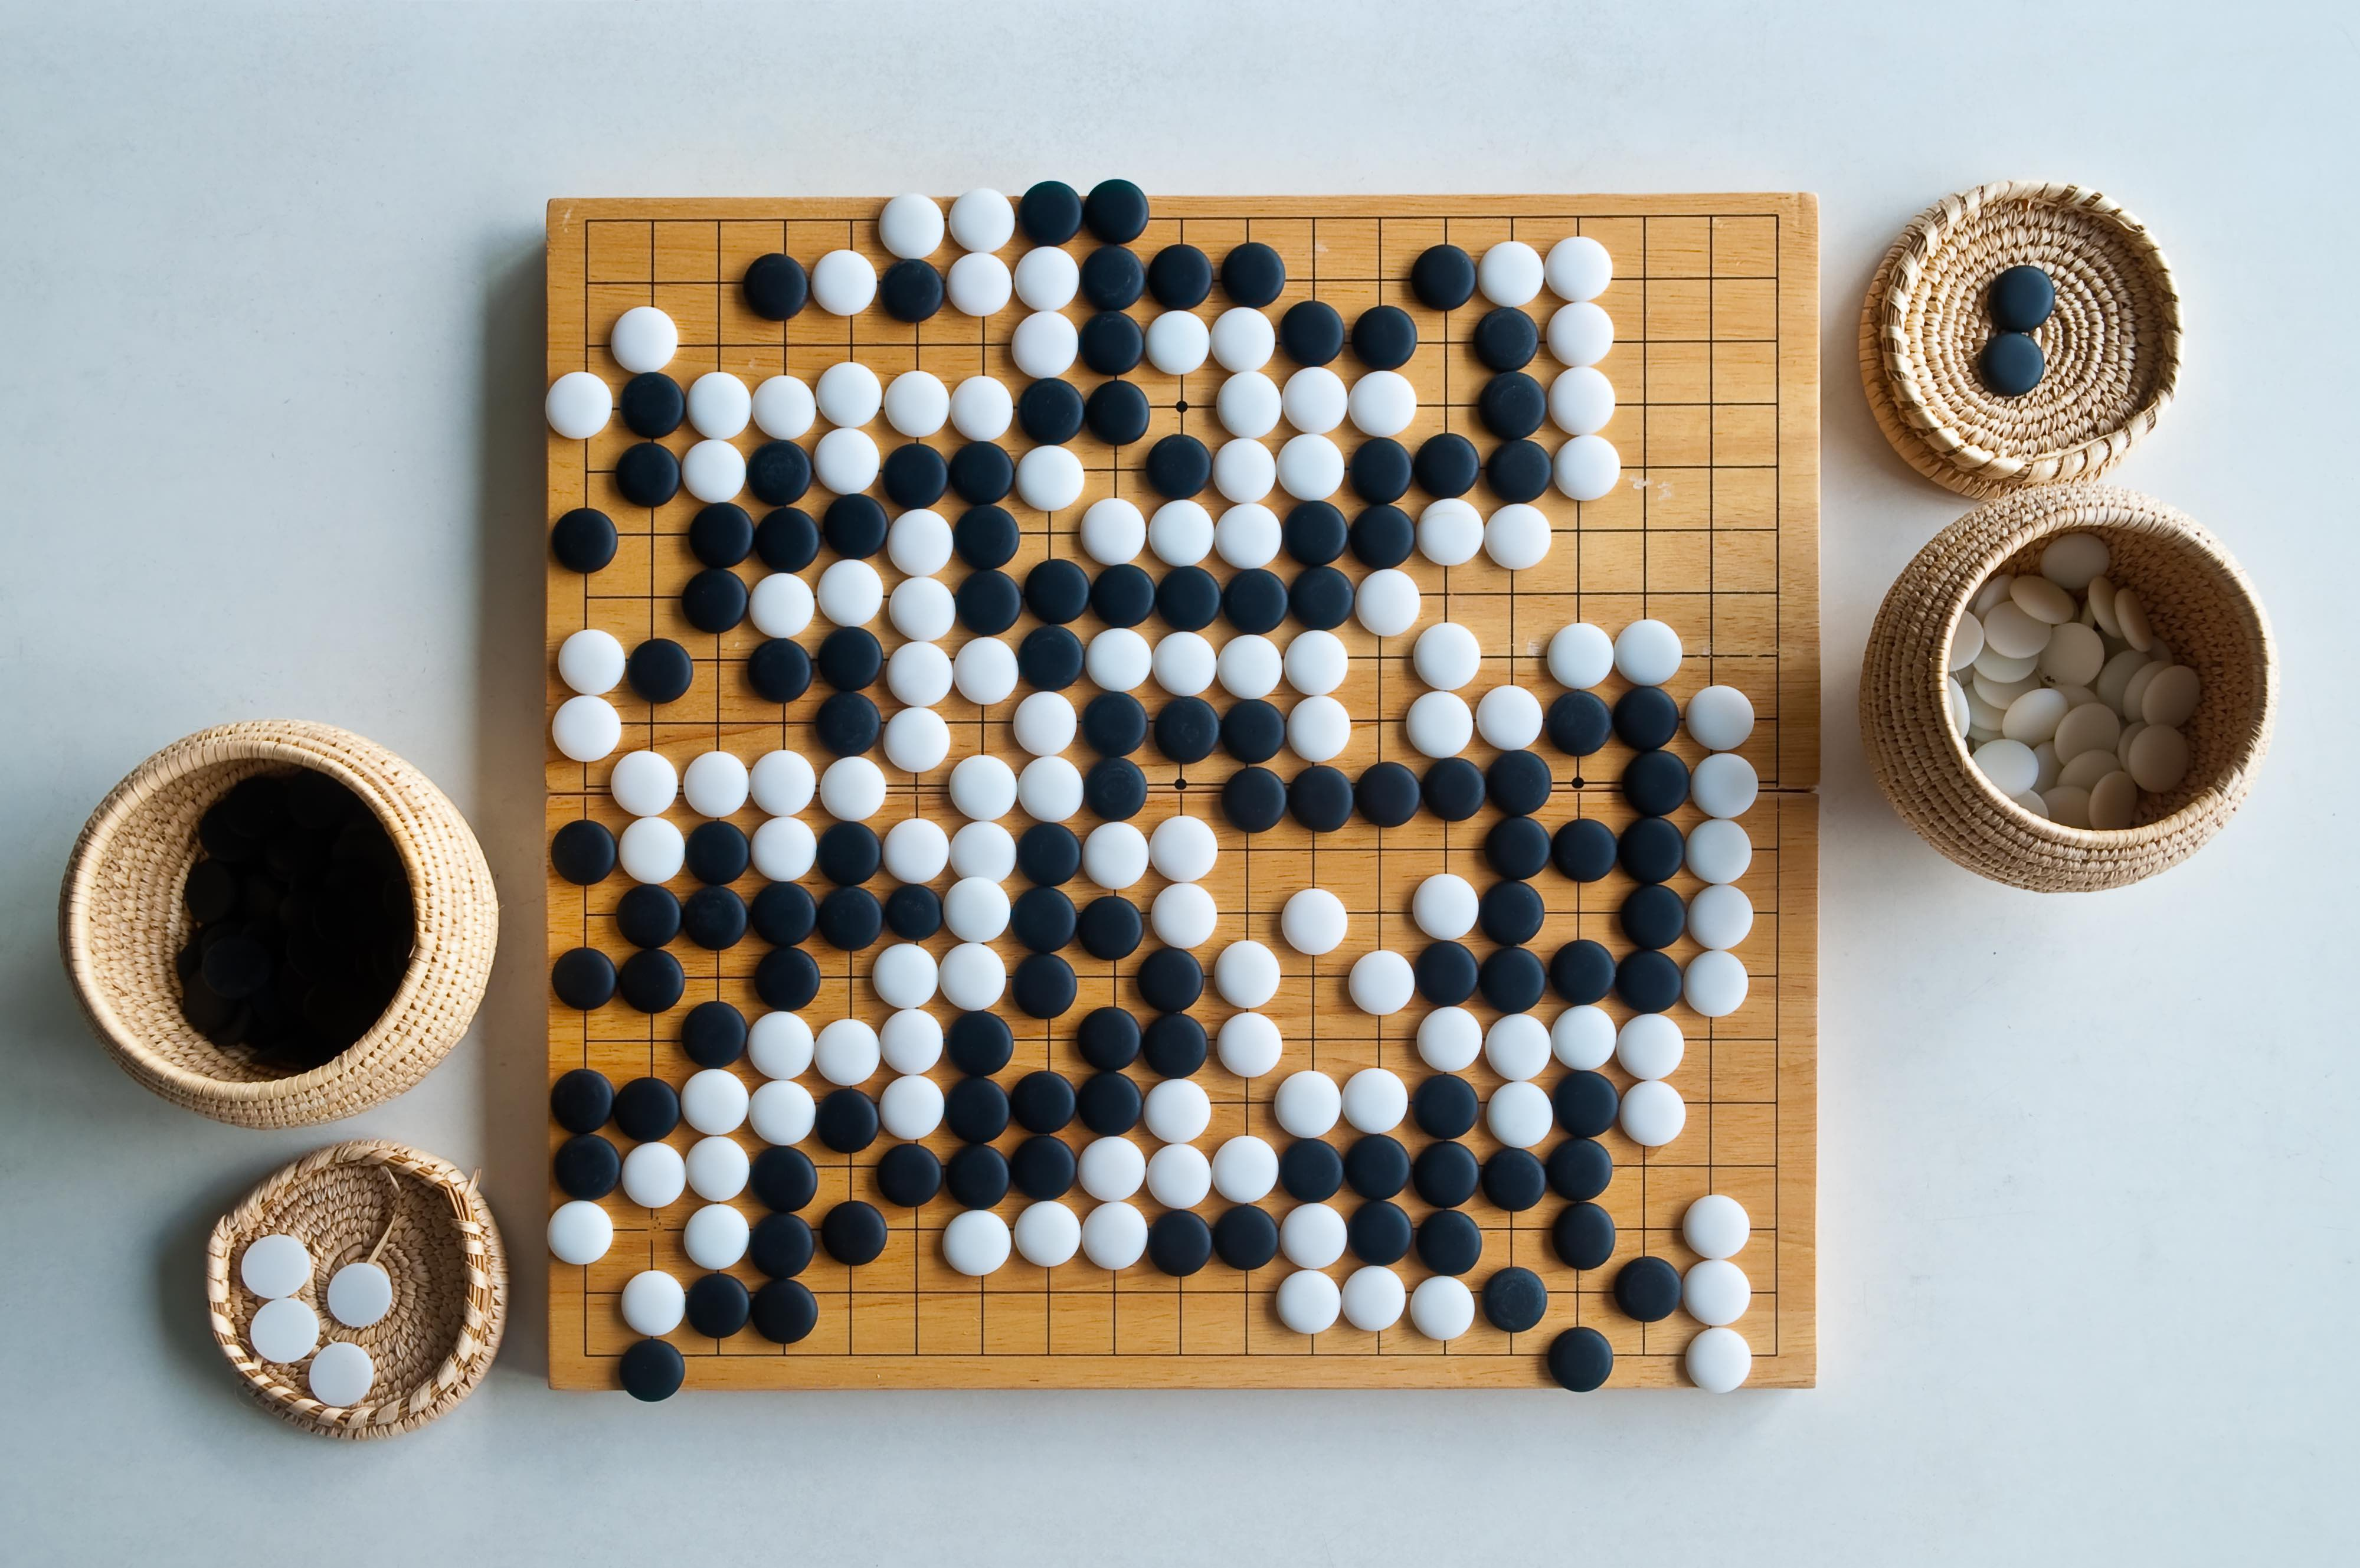
\includegraphics[scale=0.03]{../images/go.jpg}}
    \end{column}

    \begin{column}{0.5\textwidth}
      \centering{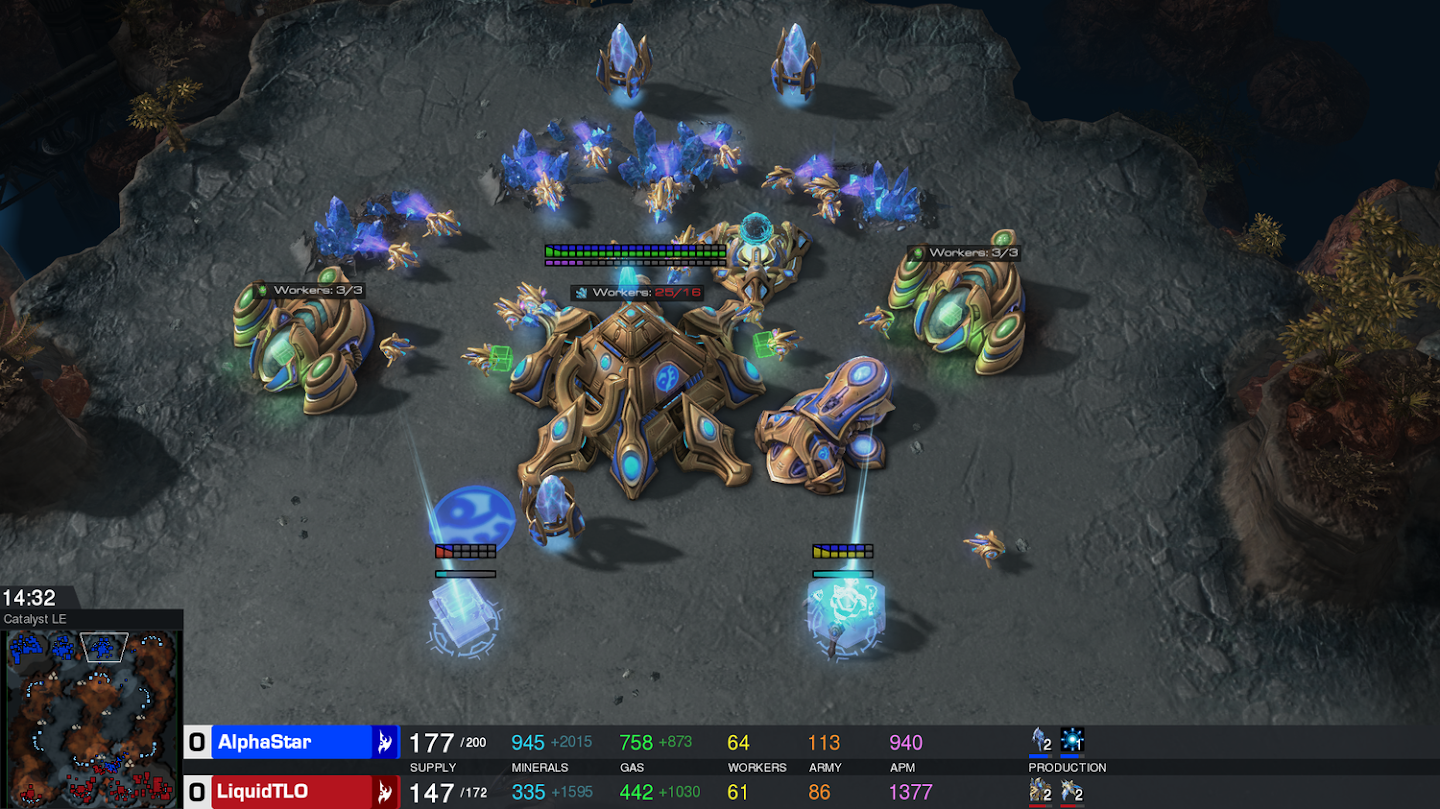
\includegraphics[scale=0.1]{../images/starcraft.png}}
    \end{column}

  \end{columns}

  \begin{itemize} 
    \item 2016 AlphaGo, \url{https://www.nature.com/articles/nature16961}
    \item 2020 MuZero, \url{https://arxiv.org/pdf/1911.08265.pdf}
    \item AlphaZero, AlphaStar ...
  \end{itemize}
\end{frame}

\begin{frame}{\bf reinforcement learning - robotics}

  \begin{columns}

    \begin{column}{0.5\textwidth}
      \centering{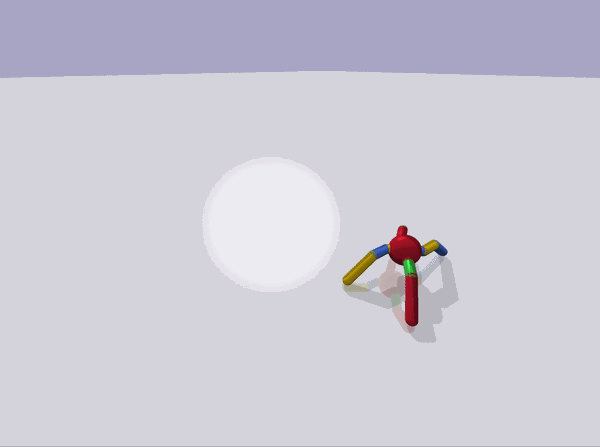
\includegraphics[scale=0.2]{../images/ant.png}}
      \centering{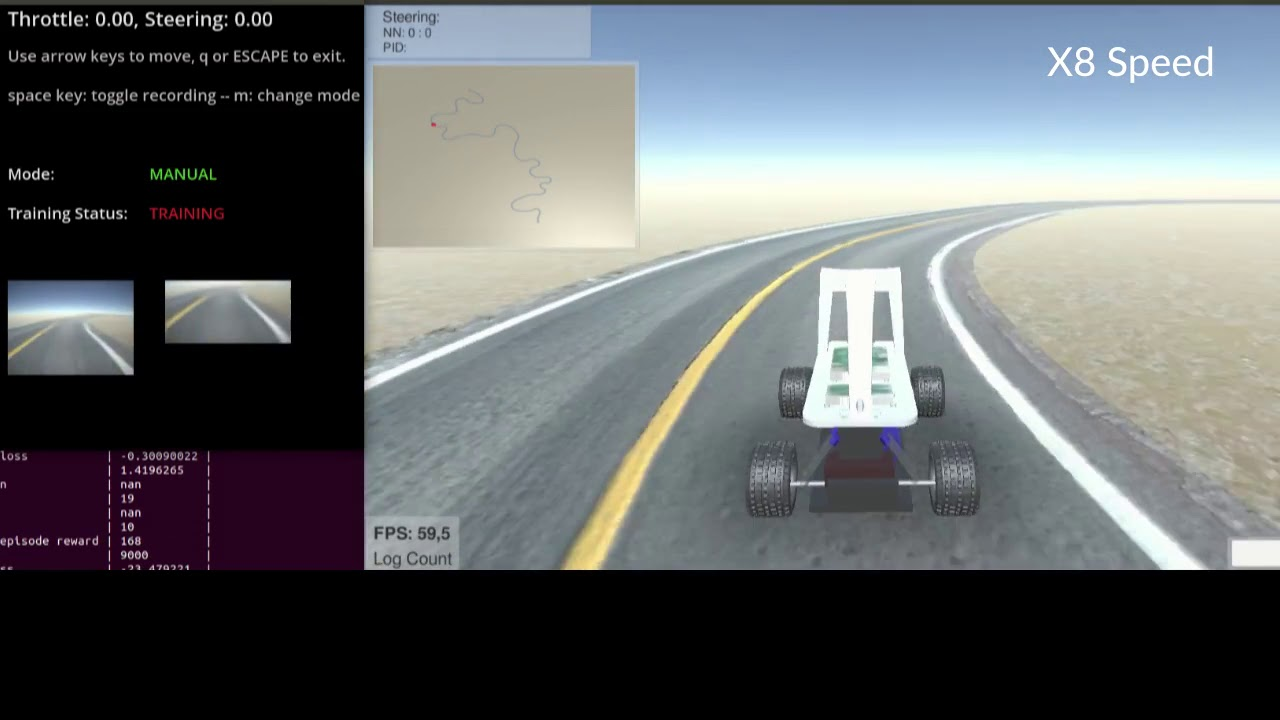
\includegraphics[scale=0.1]{../images/sac_car.jpg}}
    \end{column}

    \begin{column}{0.5\textwidth}
      \centering{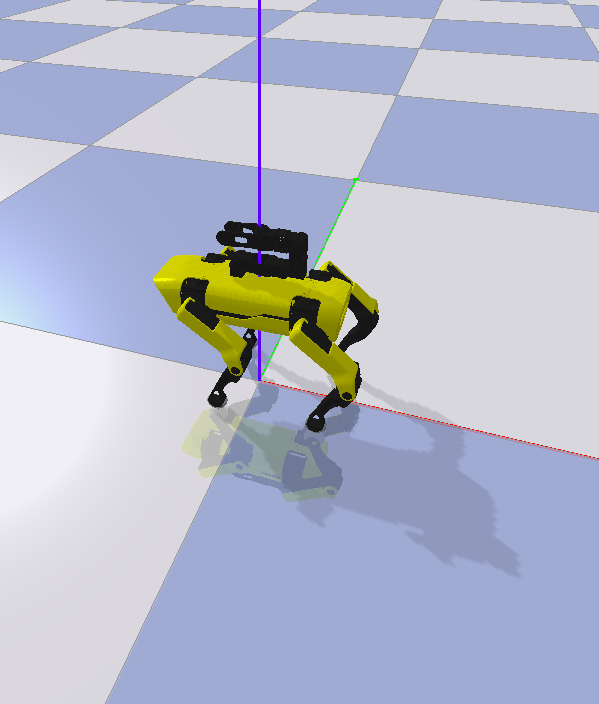
\includegraphics[scale=0.15]{../images/rex_arm.png}}
      \centering{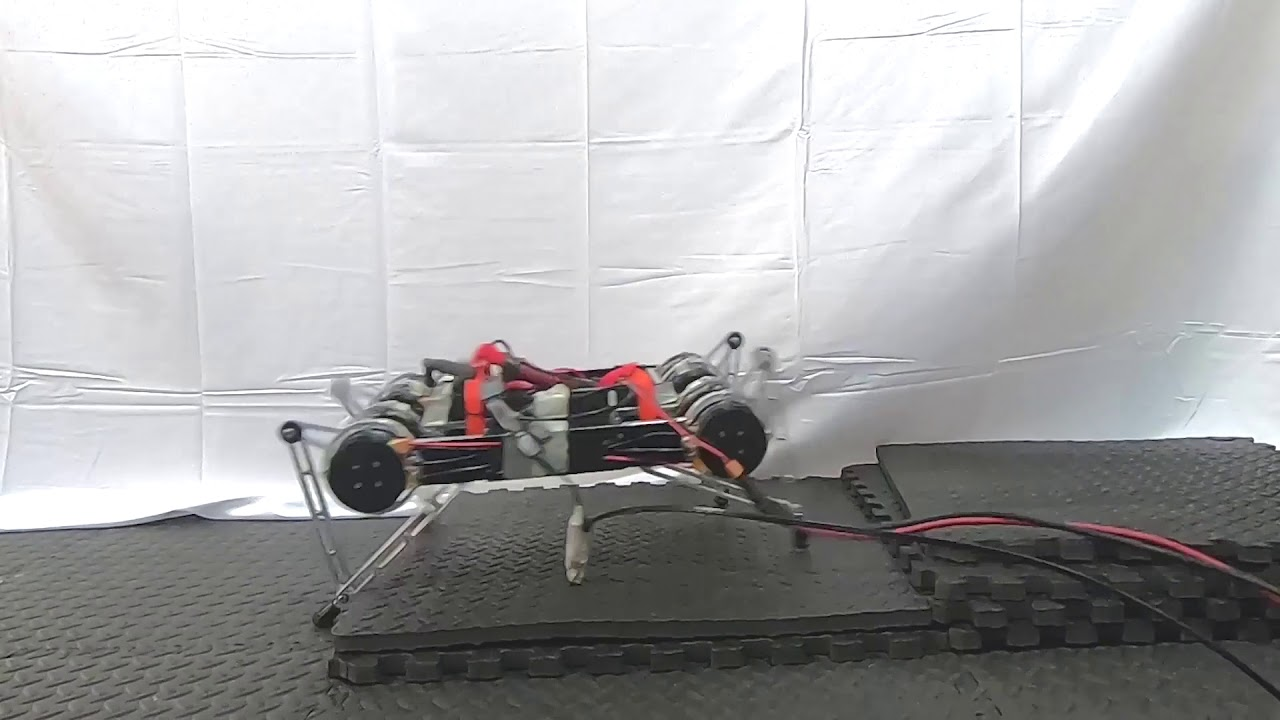
\includegraphics[scale=0.1]{../images/sac_minitaur.jpg}}
    \end{column}


  \end{columns}

\end{frame}


\begin{frame}{\bf motoko uprising - line follower}  
  \begin{columns}
    \begin{column}{0.5\textwidth}
      \centering{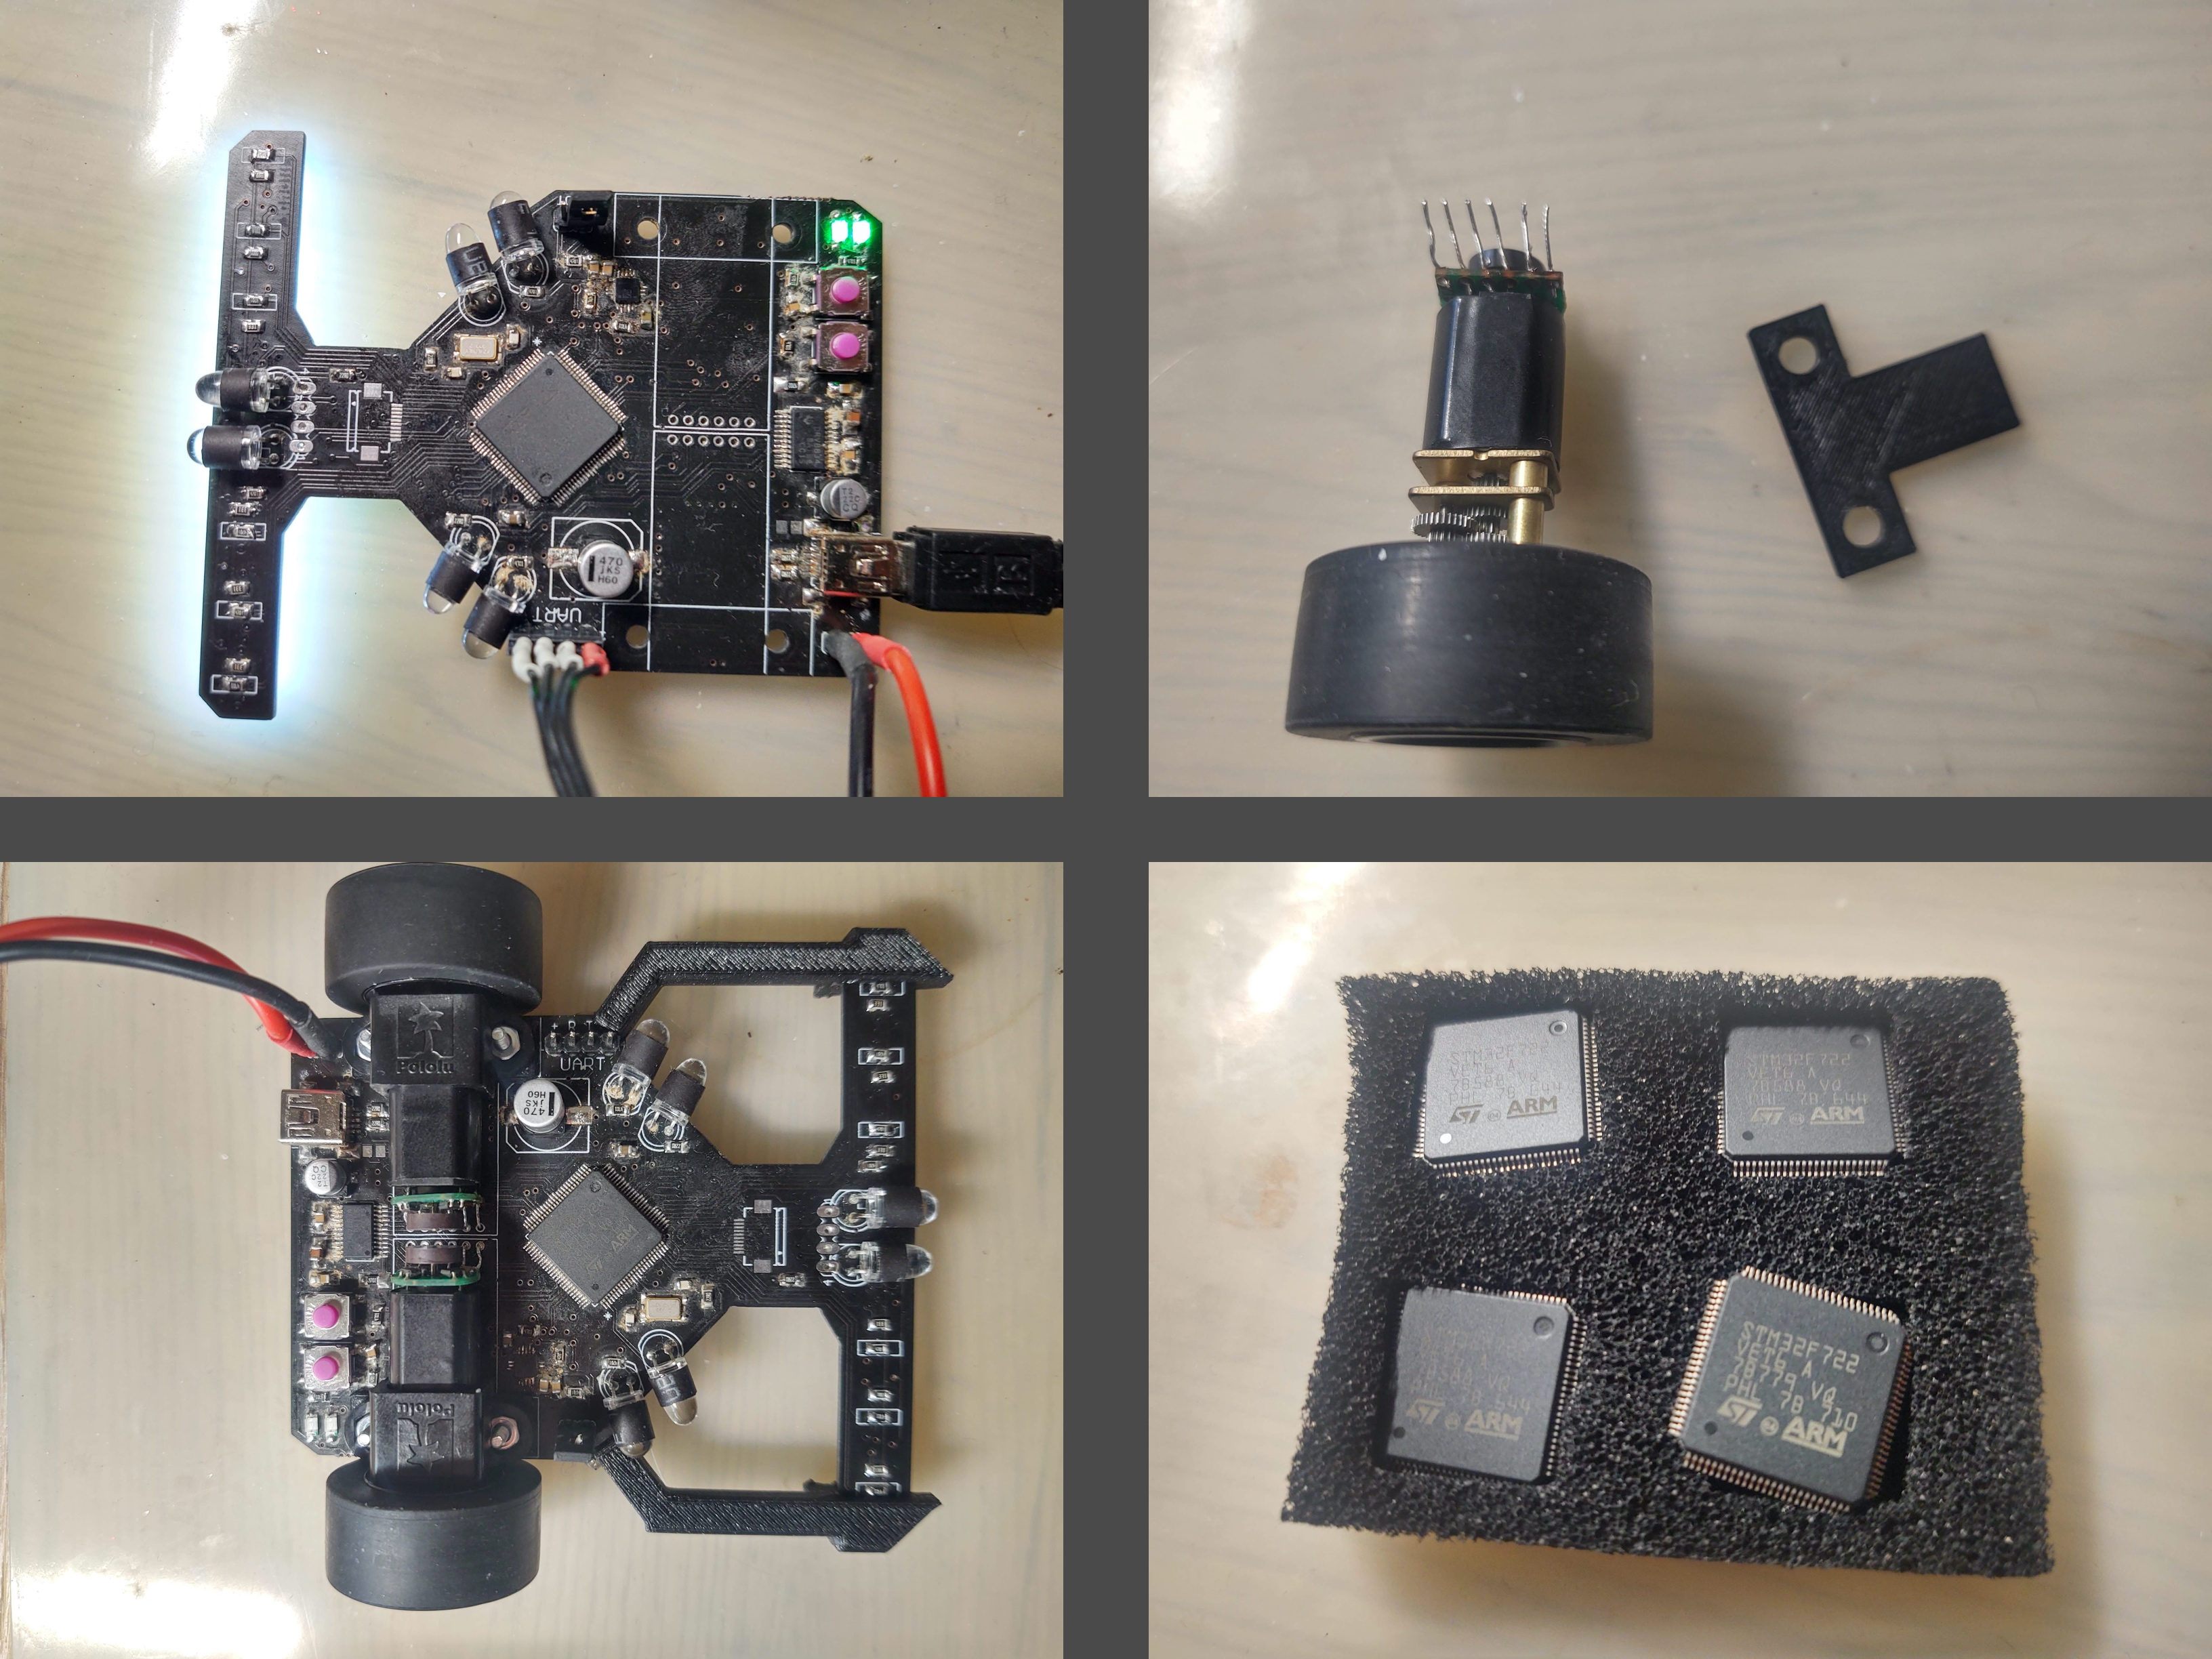
\includegraphics[scale=0.2]{../images/robot_mount.jpg}}
    \end{column}

    \begin{column}{0.5\textwidth}
      \centering{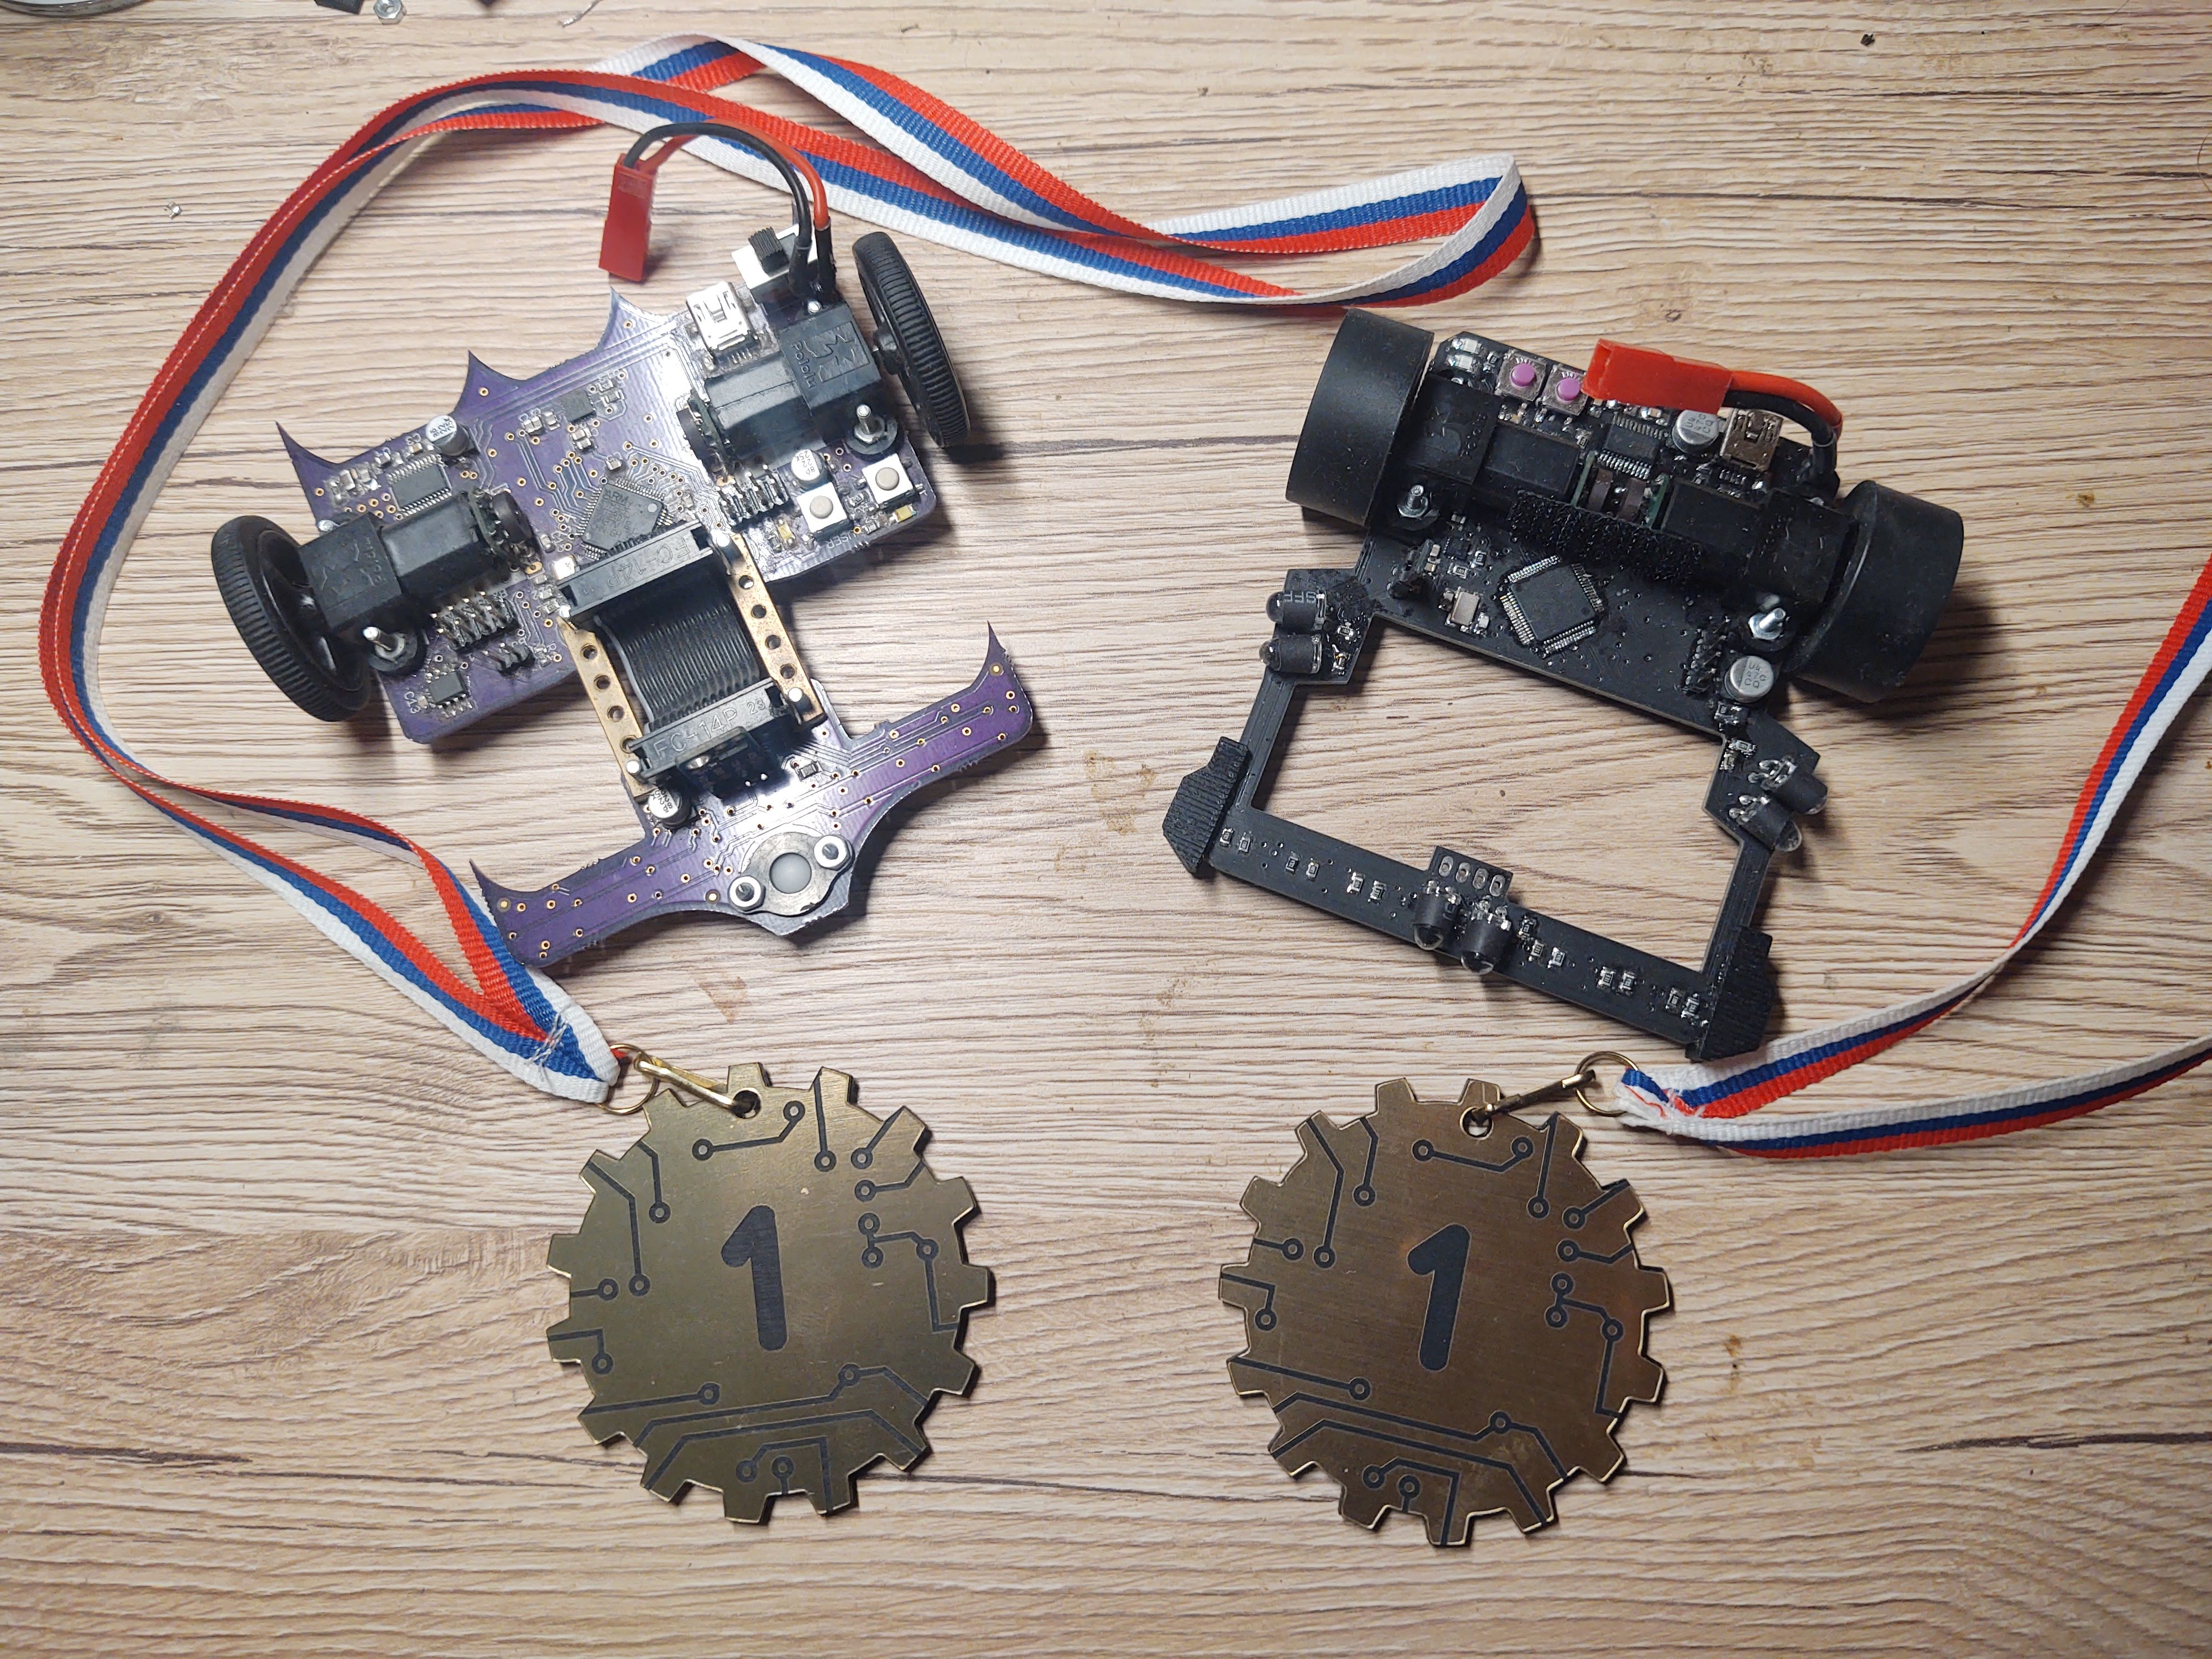
\includegraphics[scale=0.035]{../images/medals.jpg}}
    \end{column}
  \end{columns}

  video : \url{https://www.youtube.com/watch?v=xUAJ1LA6Xwc}

\end{frame}


\begin{frame}{\bf reinforcement learning}

  \begin{columns}

    \begin{column}{0.5\textwidth}
      \centering{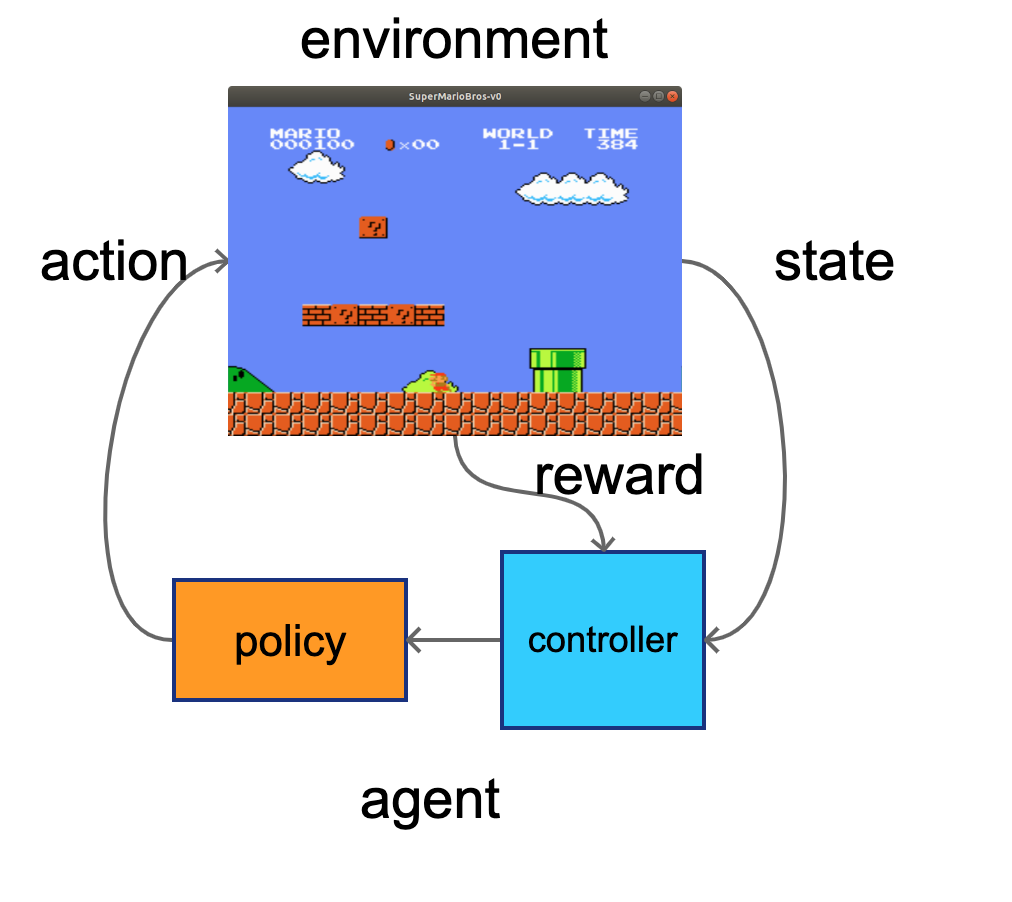
\includegraphics[scale=0.15]{../diagrams/basic/reinforcementlearning.png}}
    \end{column}

    \begin{column}{0.5\textwidth}
      \begin{itemize}
        \item obtain state
        \item select action
        \item exectute action
        \item learn from experiences
      \end{itemize}
    \end{column}

  \end{columns}

\end{frame}




\begin{frame}{\bf action space}

  \begin{itemize}
    \item discrete action space \\
      - keys, keypad
    \item continuous action space \\
      - motors, PWMs, steering, force controll
  \end{itemize}

  \centering{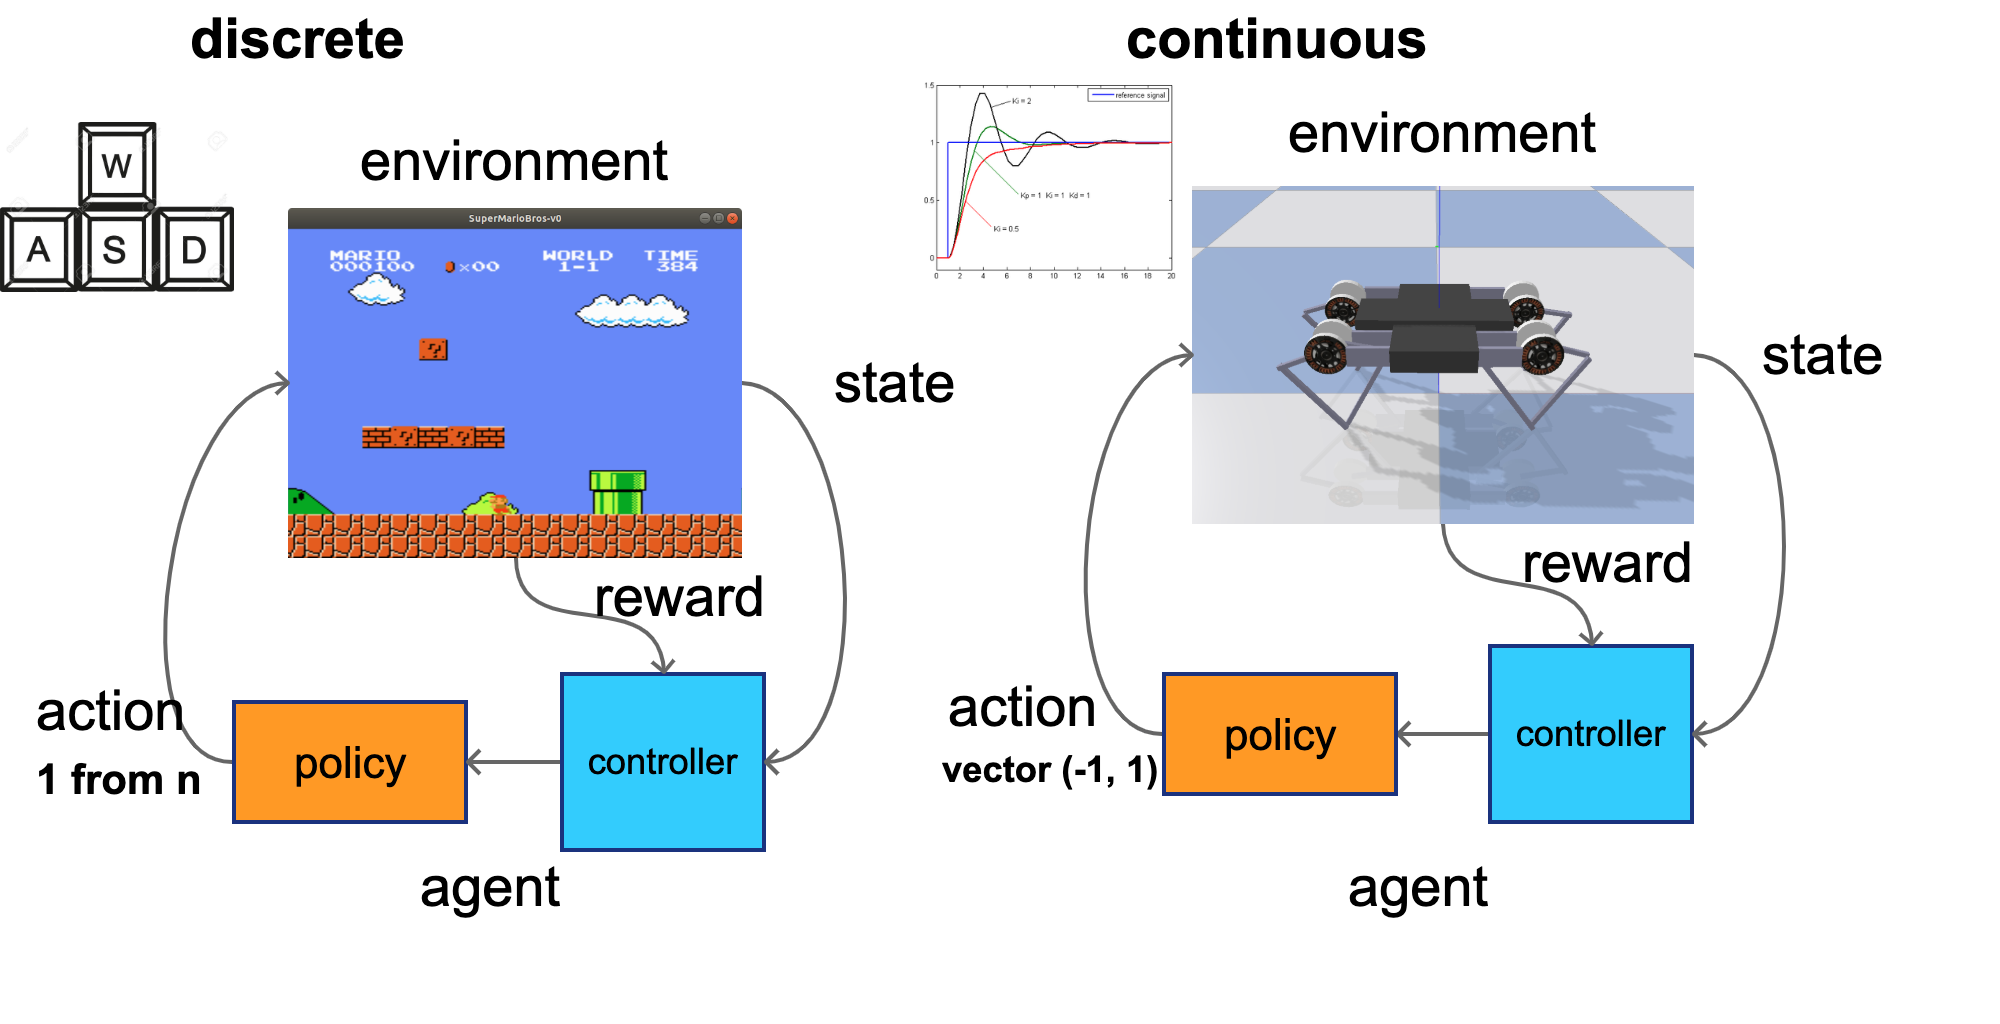
\includegraphics[scale=0.15]{../diagrams/basic/actionspace.png}}

\end{frame}


\begin{frame}{\bf deep Q learning}

  \centering{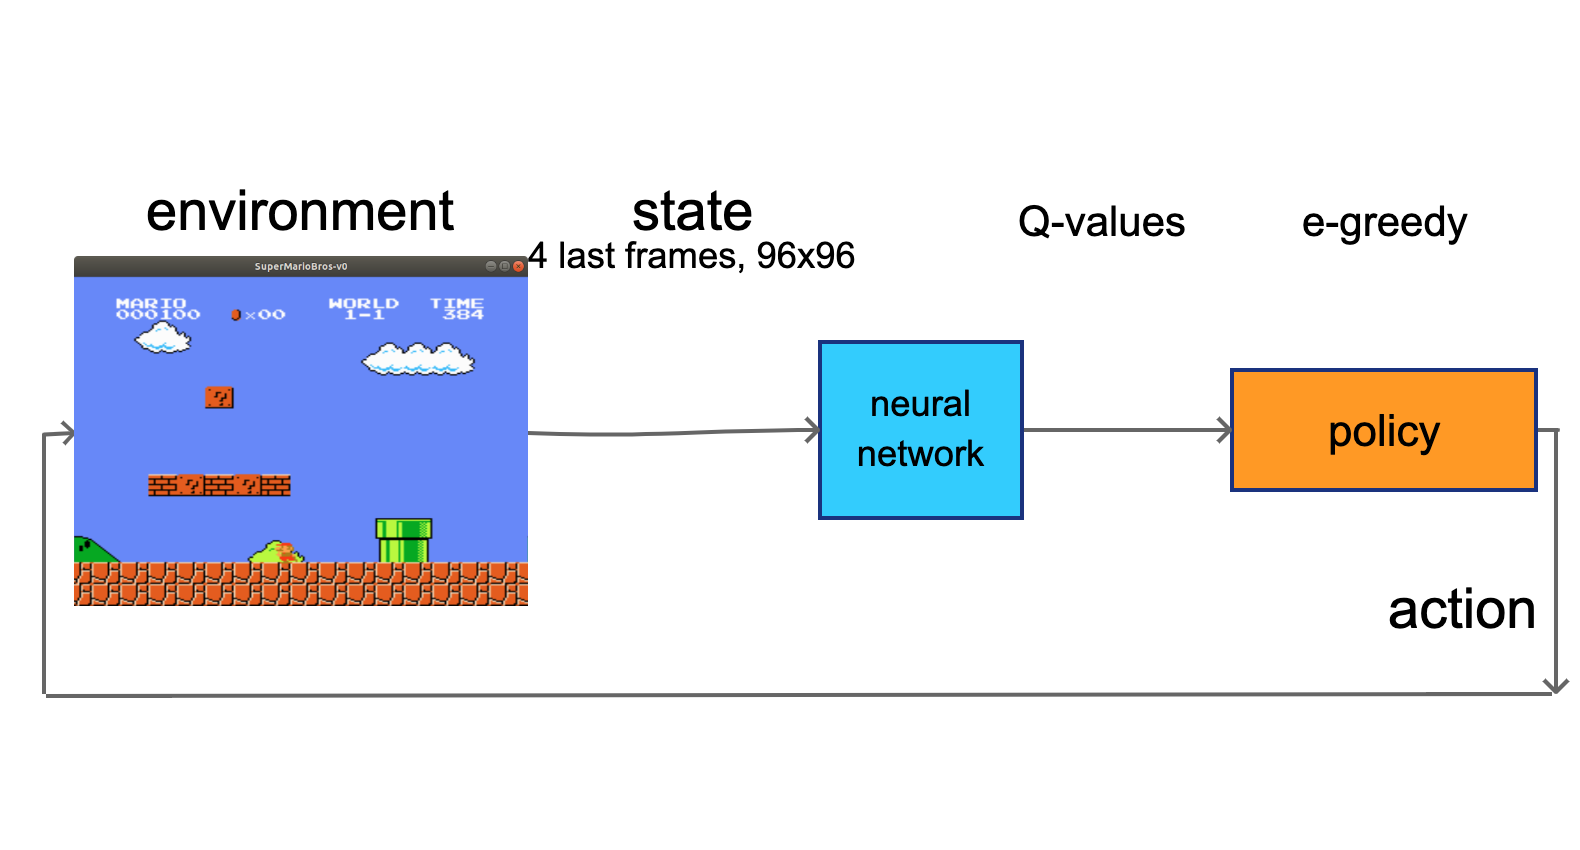
\includegraphics[scale=0.15]{../diagrams/basic/deepqnetwork.png}}

  \begin{enumerate}
    \item play games
    \item store transitions into buffer \\
      - state, action, reward, done
    \item learn from buffer
  \end{enumerate}
\end{frame}


\begin{frame}{\bf deep Q learning}

  \centering{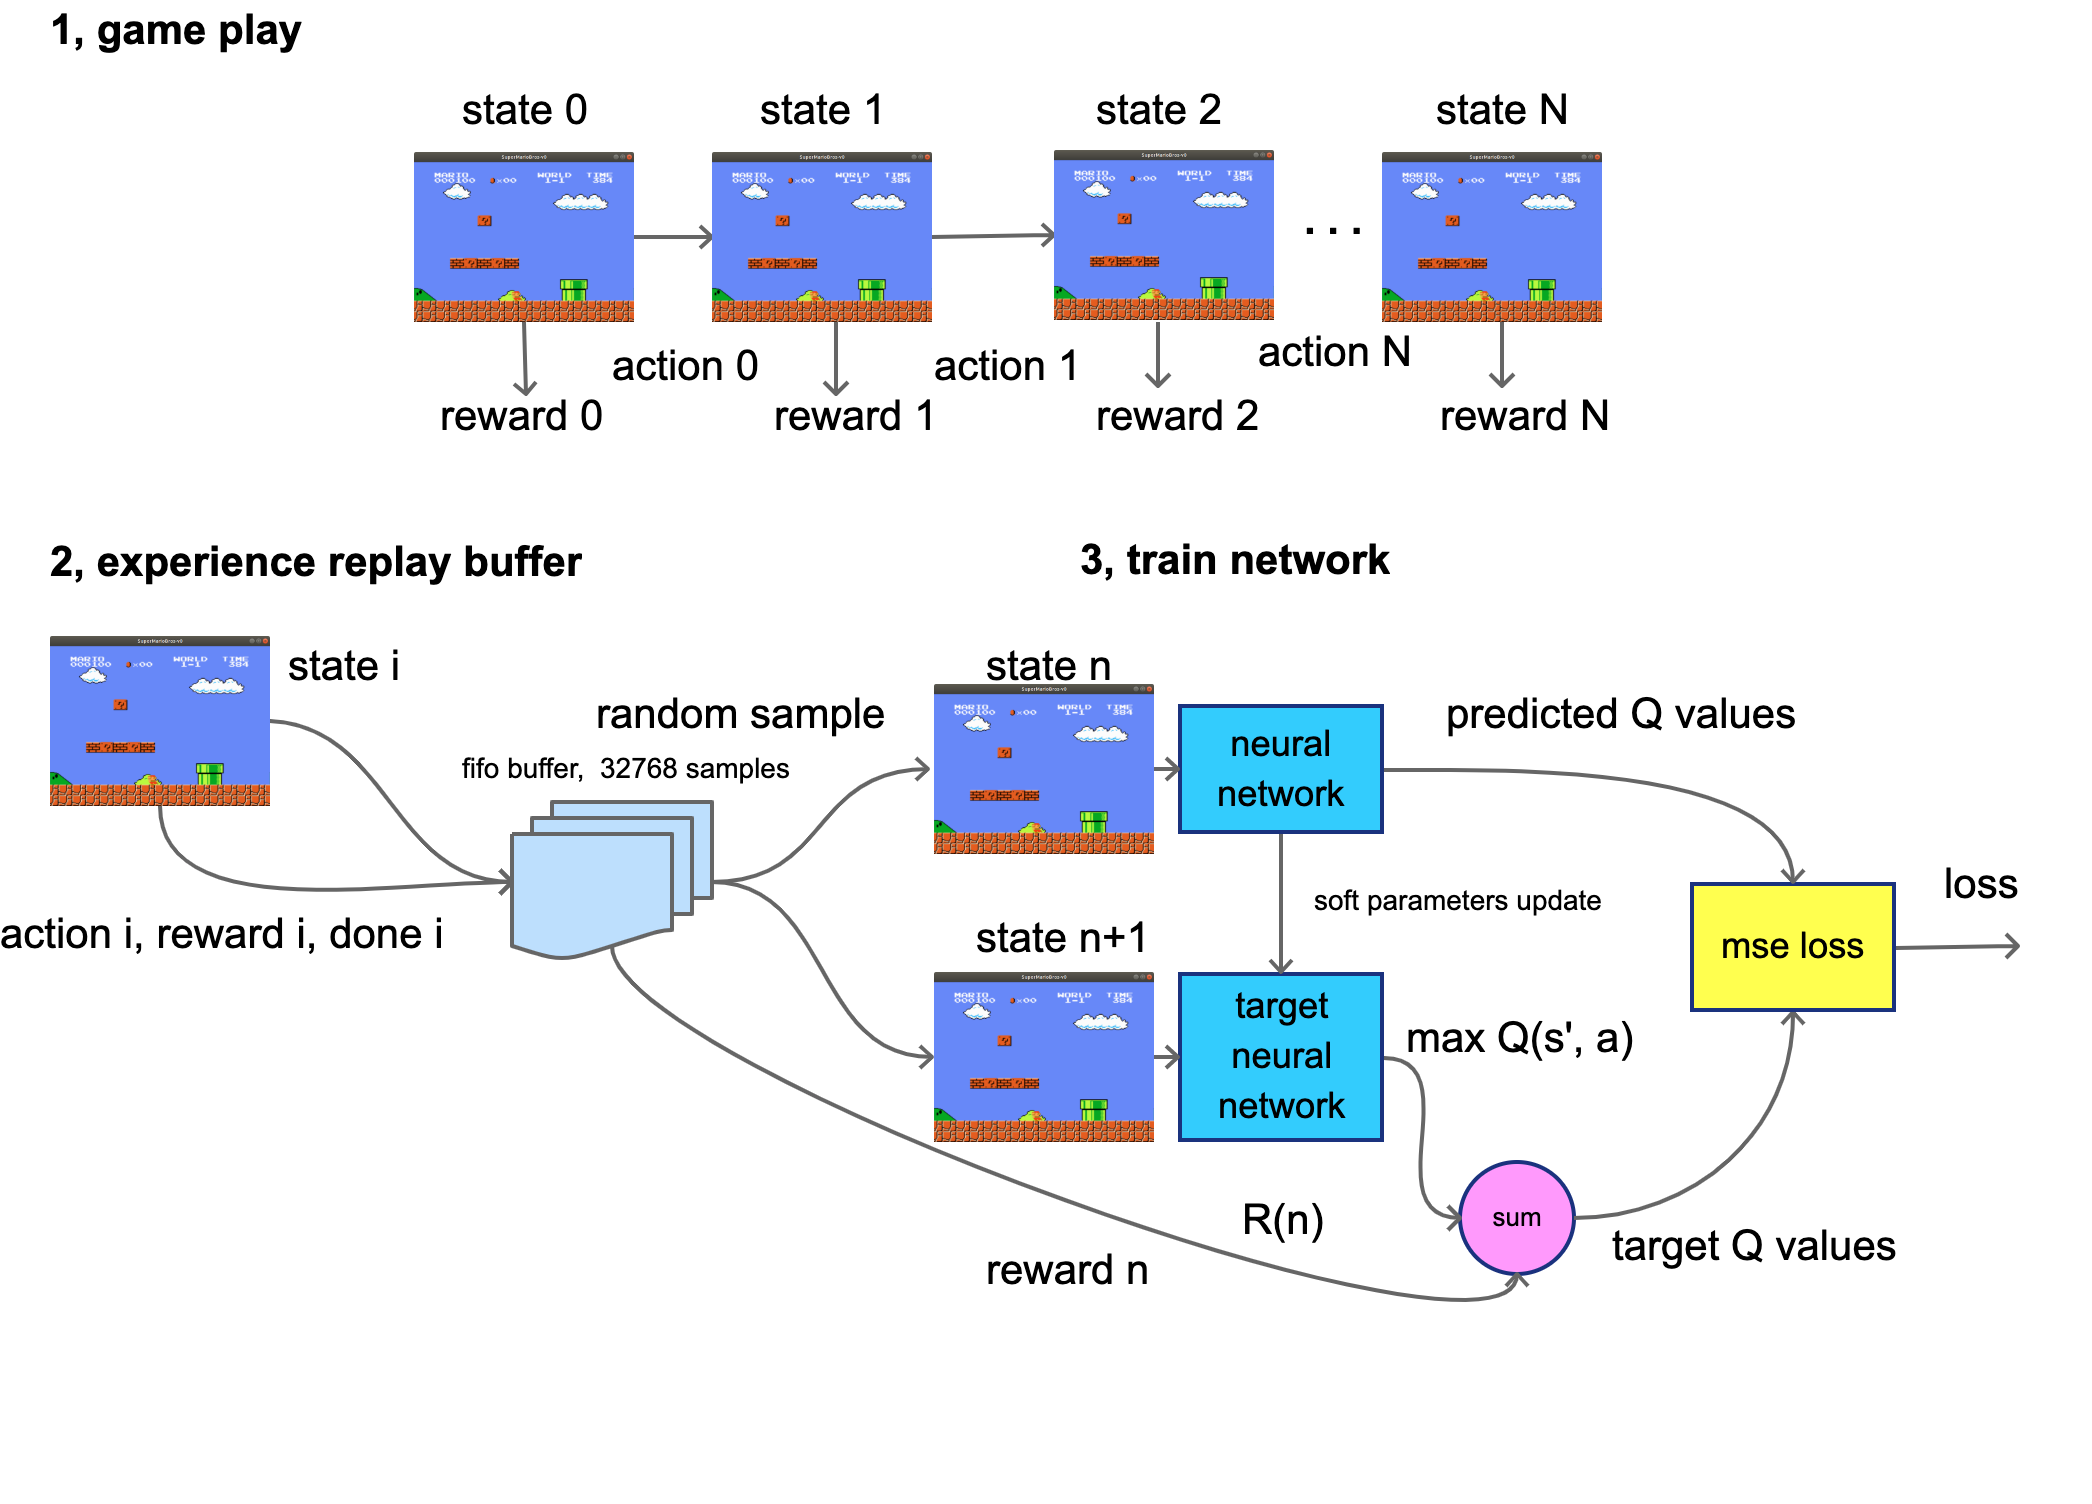
\includegraphics[scale=0.15]{../diagrams/basic/deepqlearning.png}}

\end{frame}


\begin{frame}{\bf deep Q learning}

  \centering{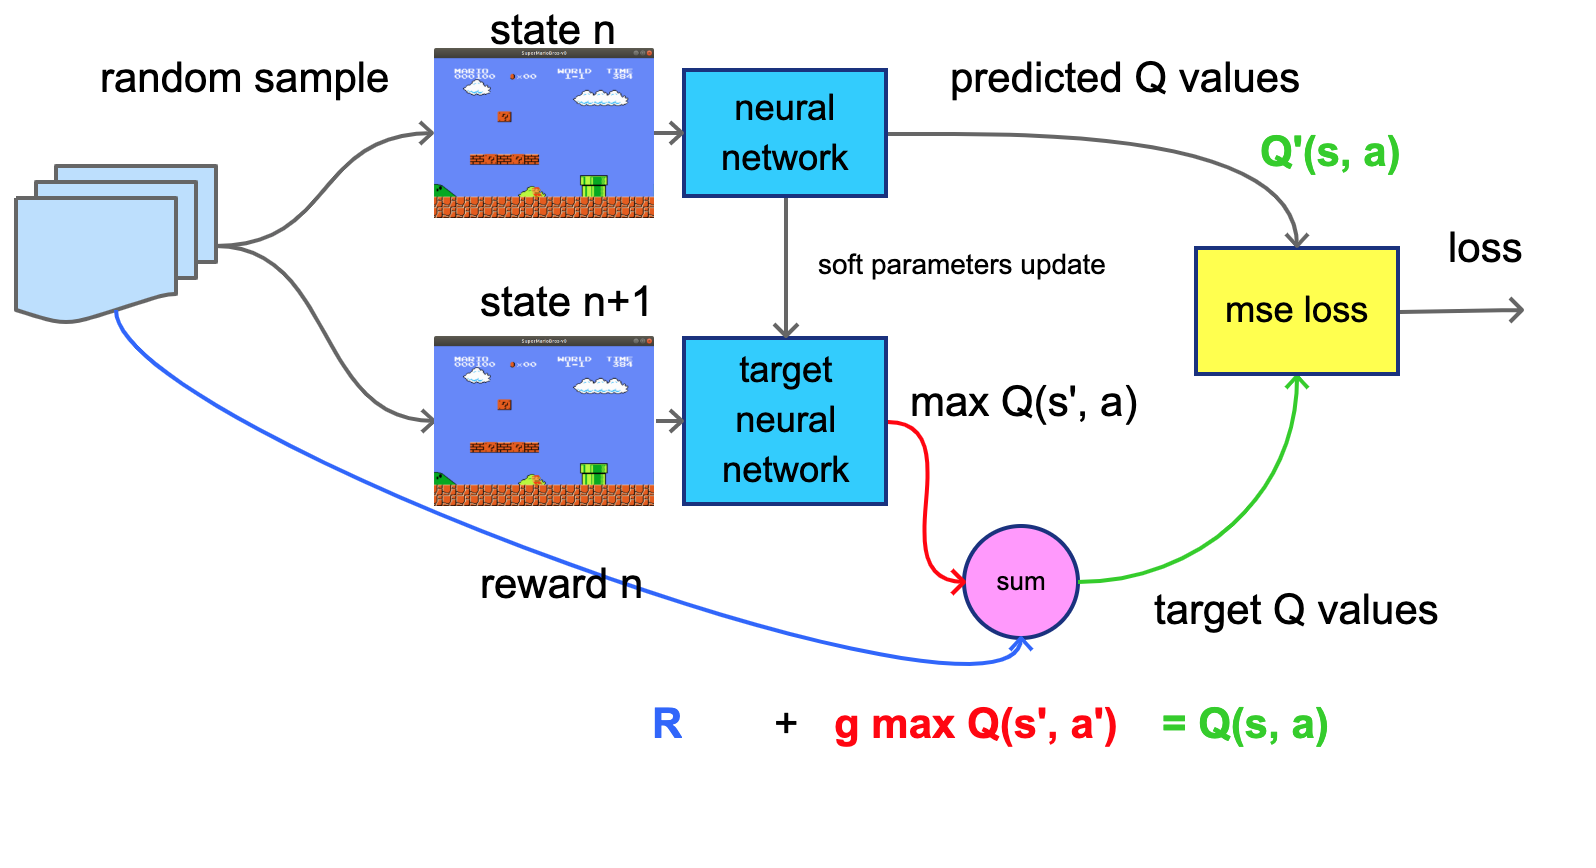
\includegraphics[scale=0.15]{../diagrams/basic/deepqlearningdetail.png}}

  \begin{align*}
    Q(s, a; \theta) = \underset{\textcolor{cyan}{reward}}{R} + \underset{\textcolor{OrangeRed}{discounted\ future\ reward}}{\gamma \max \limits_{a'} Q(s', a'; \theta^-)}
  \end{align*}

  \begin{align*}
    \mathcal{L(\theta)} = \left( R + \gamma \max \limits_{a'} Q(s', a'; \theta^-) - Q(s, a; \theta)  \right)^2
  \end{align*}
\end{frame}


\begin{frame}{\bf deep Q learning}

  \centering{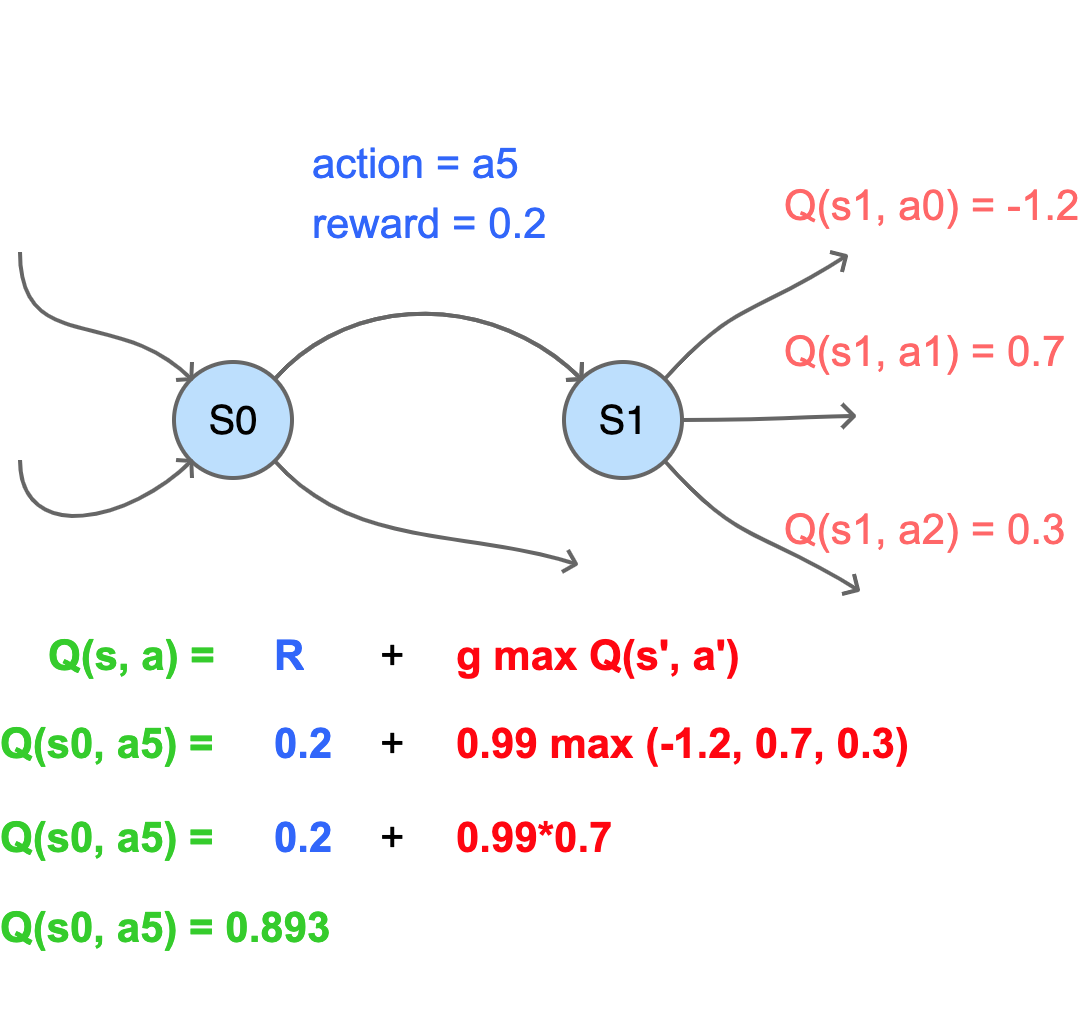
\includegraphics[scale=0.12]{../diagrams/basic/qlearning.png}}

  \begin{align*}
    Q(s, a; \theta) = \underset{\textcolor{cyan}{reward}}{R} + \underset{\textcolor{OrangeRed}{discounted\ future\ reward}}{\gamma \max \limits_{a'} Q(s', a'; \theta^-)}
  \end{align*}

  \begin{align*}
    \mathcal{L(\theta)} = \left( R + \gamma \max \limits_{a'} Q(s', a'; \theta^-) - Q(s, a; \theta)  \right)^2
  \end{align*}
\end{frame}



\begin{frame}{\bf model architecture}

  \centering{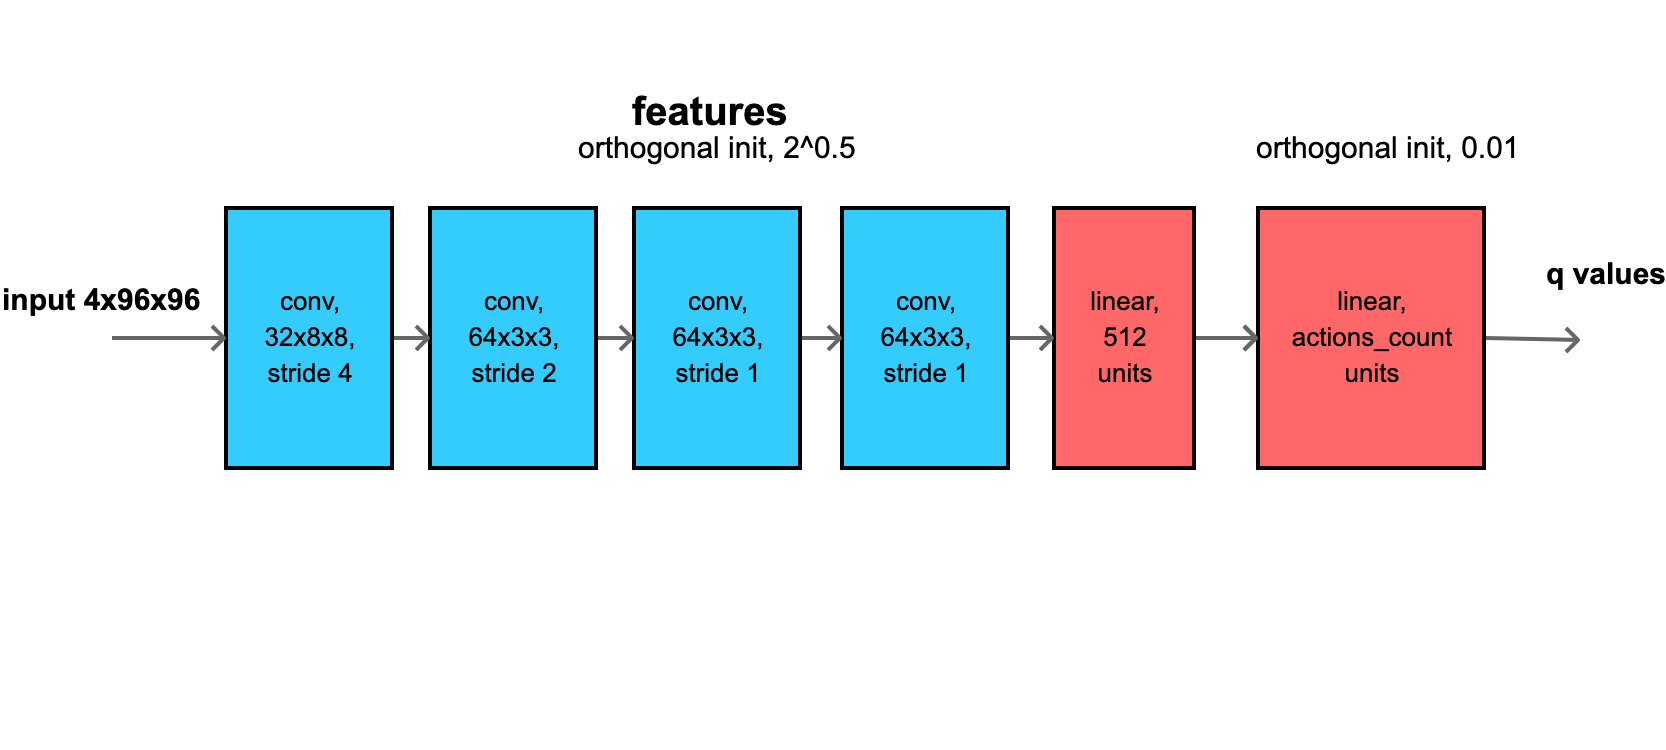
\includegraphics[scale=0.15]{../diagrams/models/dqncnn.png}}

  \begin{itemize}
    \item input 96x96 grayscale, 4 stacked frames
    \item 8x8 and 3x3 convs, with strides
    \item two fully connected layers
    \item small learning rate $\eta = 0.0001$, batch size = 32
    \item $\gamma = 0.99$
    \item exploration $\epsilon$-greedy, 1M samples linear decay from 1 to 0.05
    \item total training 8..16M samples
  \end{itemize}
 
\end{frame}

\begin{frame}{\bf dueling DQN, model architecture}

  \centering{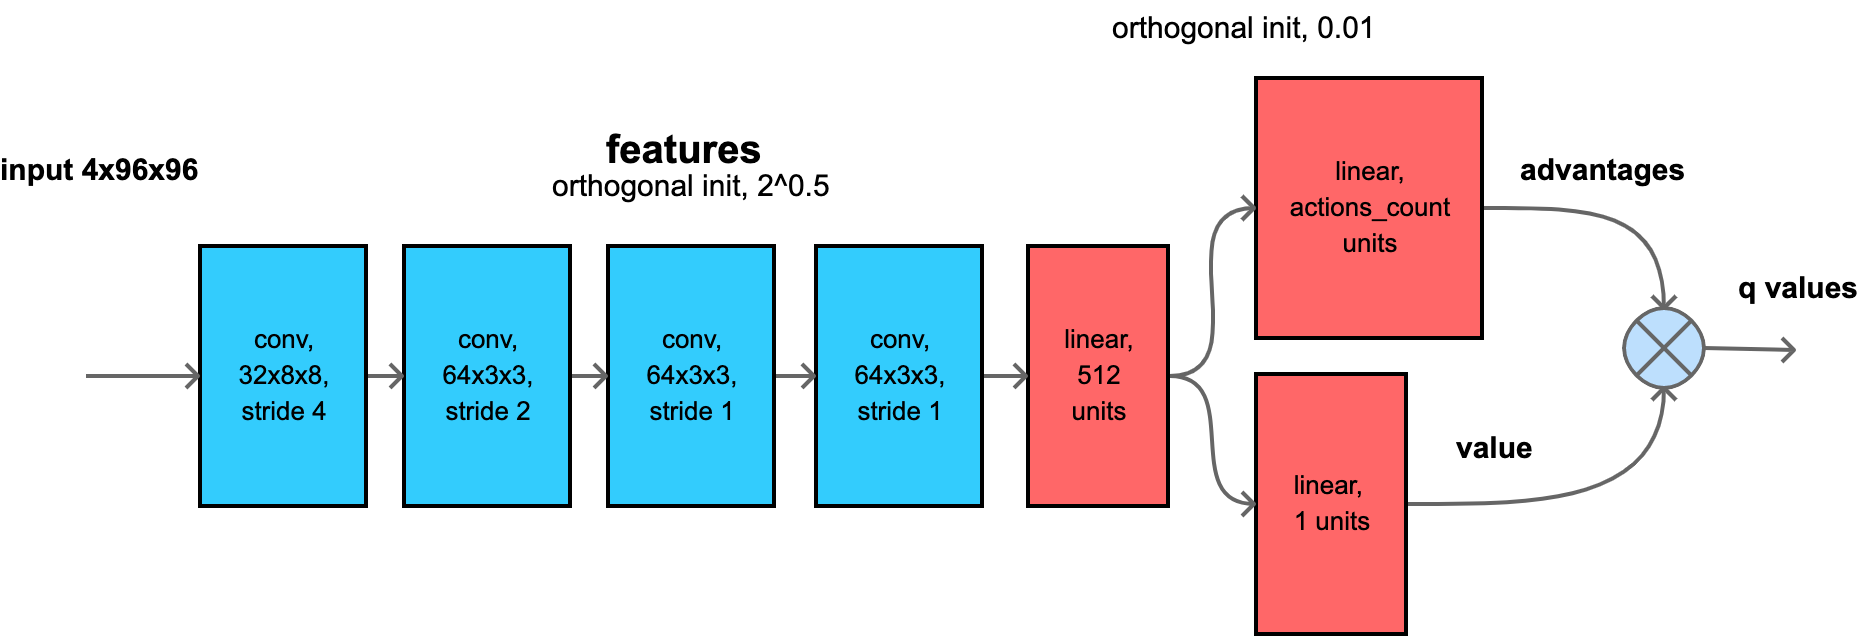
\includegraphics[scale=0.15]{../diagrams/models/duelingdqncnn.png}}

  \begin{align*}
    Q(s, a) &= V(s) + A(s, a) \\
    Q(s, a) &= V(s) + A(s, a) - \frac{1}{|\mathcal{A}|}\sum_{a' \in \mathcal{A}}A(s, a')
  \end{align*}

  \centering{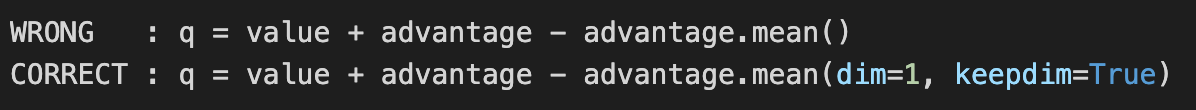
\includegraphics[scale=0.5]{../images/dueling_dqn_code.png}}

\end{frame}


\begin{frame}{\bf DDPG}

  {\bf deep deterministic policy gradietnt}

  \begin{itemize}
    \item continuous action space
    \item natural extension of DQN
    \item actor-critic structure
  \end{itemize}

  \centering{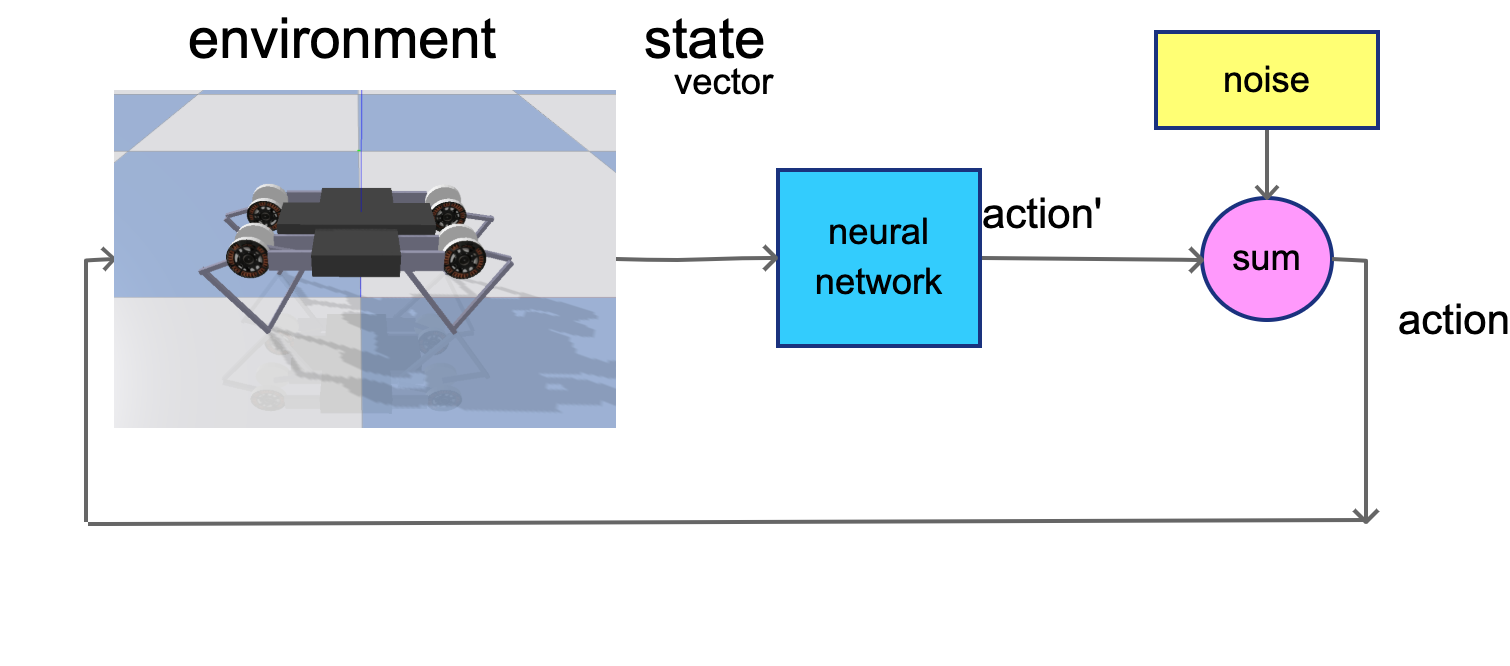
\includegraphics[scale=0.15]{../diagrams/basic/ddpgnetwork.png}}

\end{frame}




\begin{frame}{\bf DDPG}

  \centering{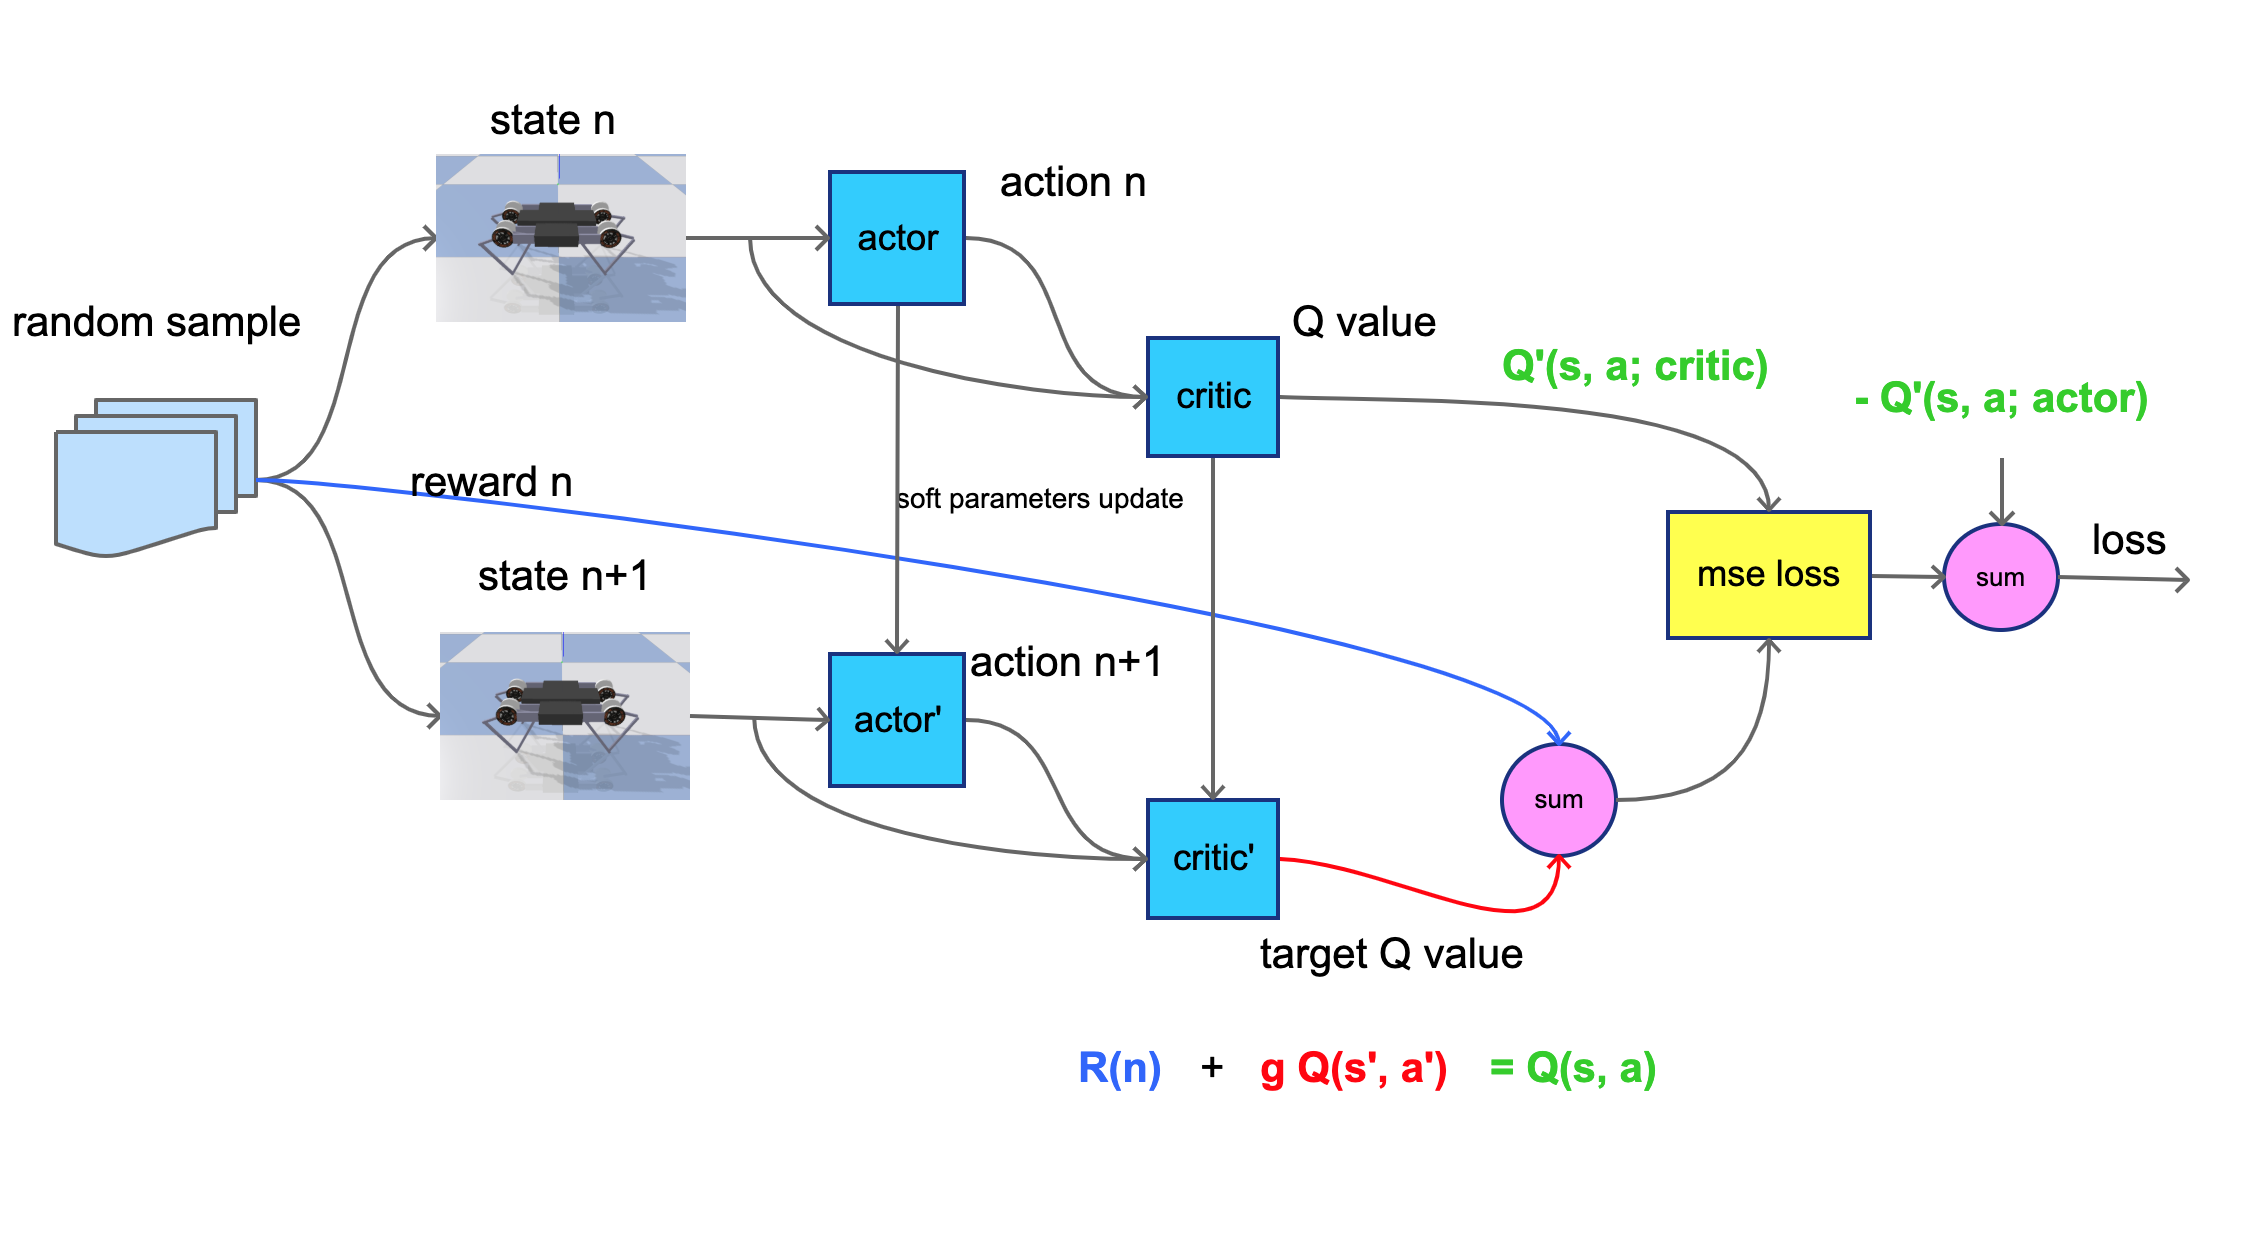
\includegraphics[scale=0.12]{../diagrams/basic/ddpgtraining.png}}

\end{frame}


\begin{frame}{\bf DDPG}

  \centering{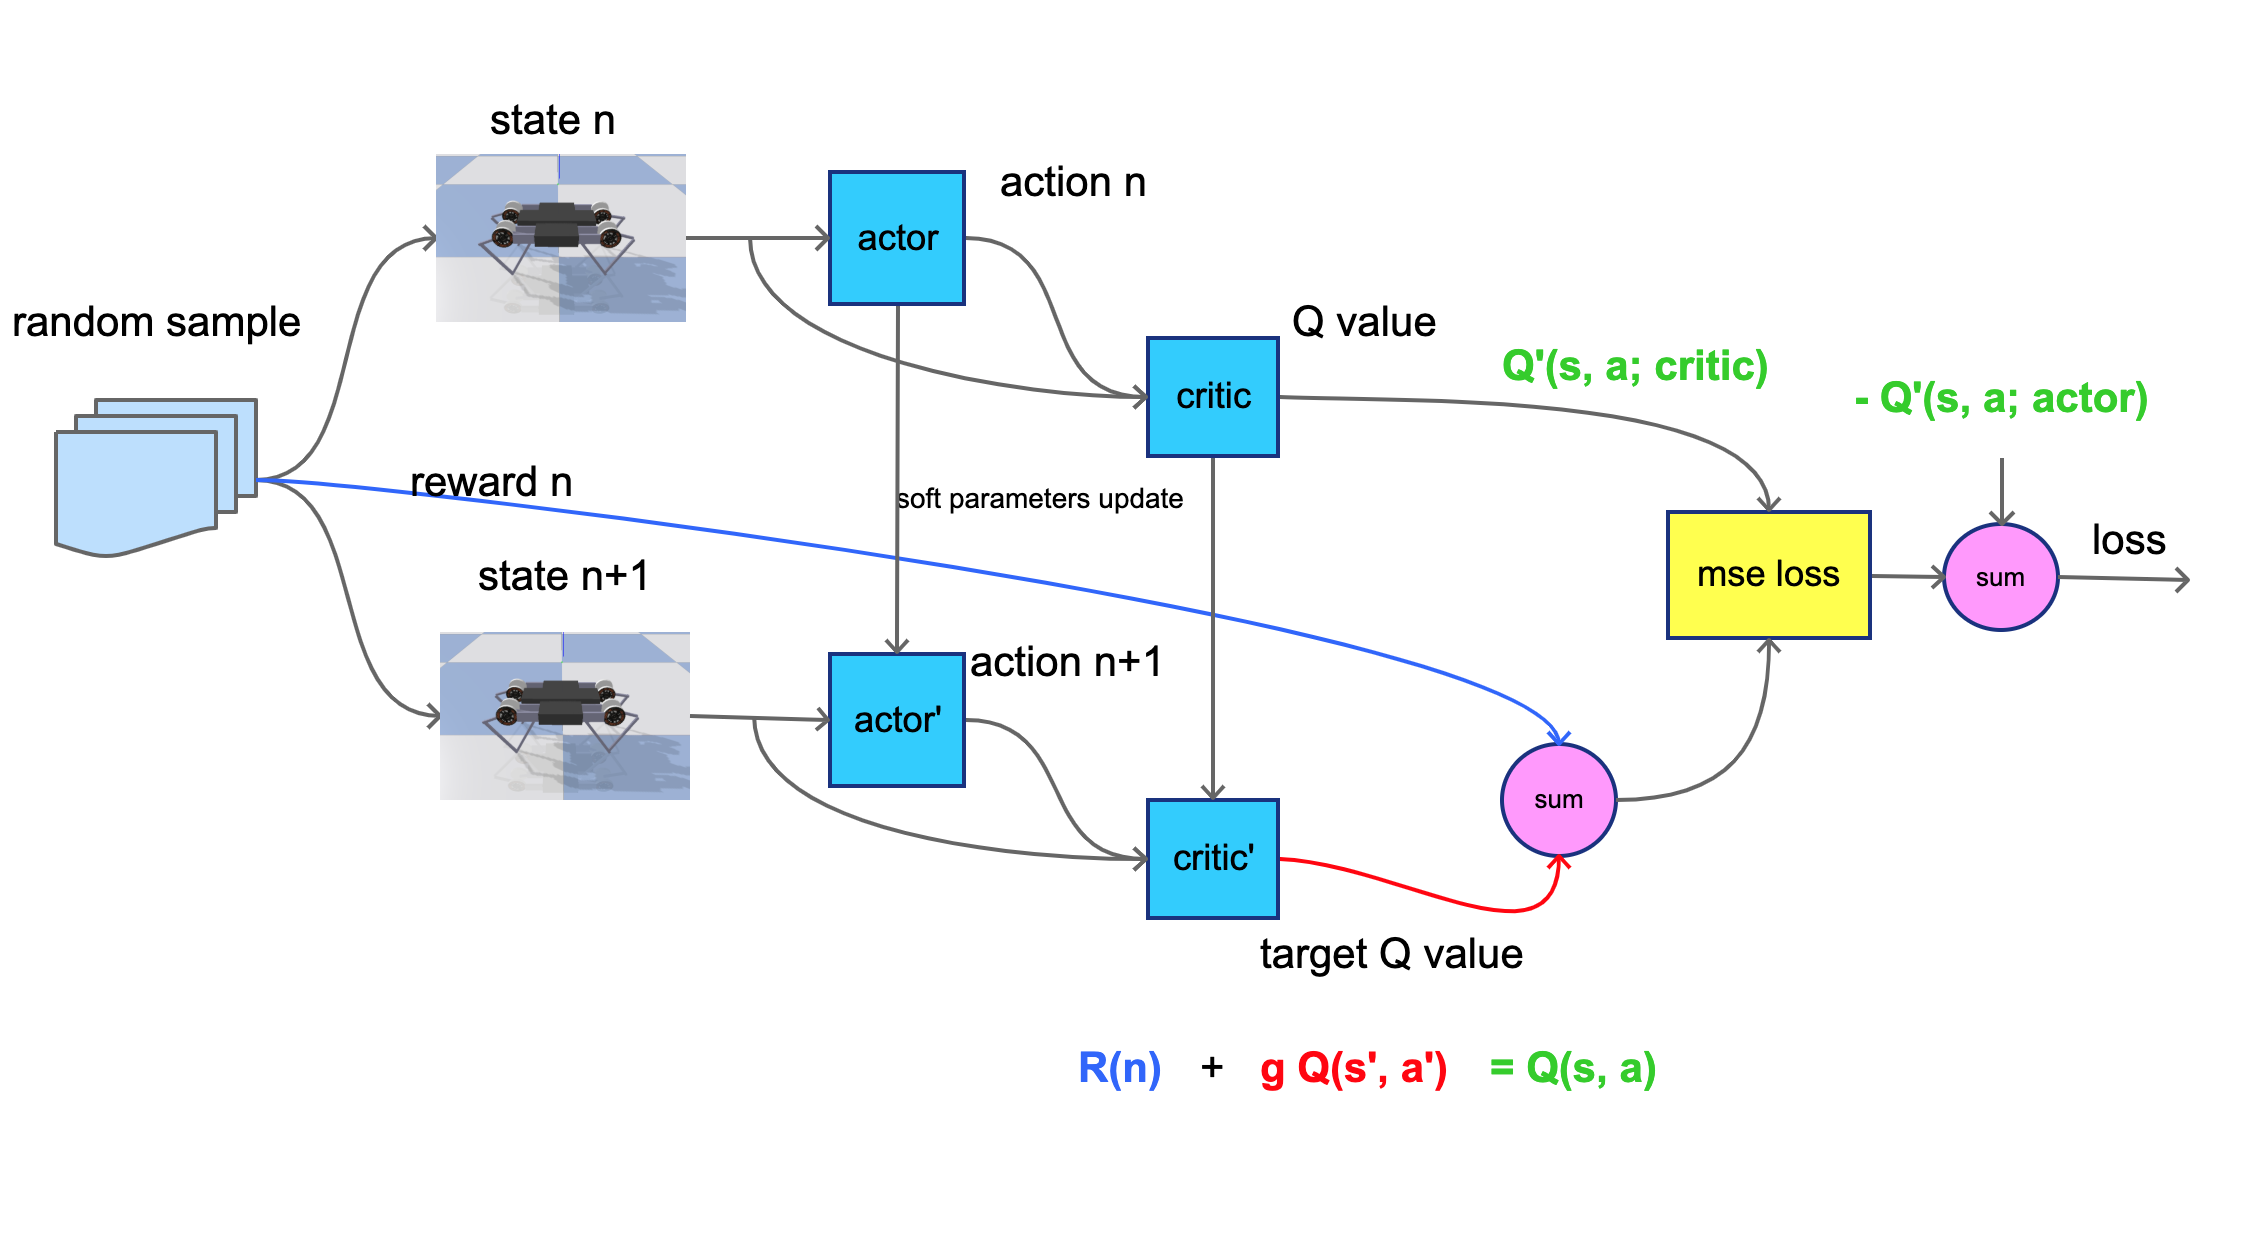
\includegraphics[scale=0.08]{../diagrams/basic/ddpgtraining.png}}

  \begin{align*}
    \mathcal{L(\theta)} &= \left( R + \gamma Q(s', A(s'; \phi^-); \theta^-) - Q(s, A(s; \phi); \theta)  \right)^2 \\
    \mathcal{L(\phi)} &= -Q(s, A(s; \phi); \theta)
  \end{align*}

  where
  \begin{itemize}
    \item $Q$ is critic network with parameters $\theta$
    \item $A$ is actor network with parameters $\phi$
  \end{itemize}
  
\end{frame}


\begin{frame}{\bf reinforcement learning - algorithms}
   \begin{itemize}
    \item discrete actions space

        \begin{itemize}
          \item Deep Q-network, DQN
          \item Dueling DQN
          \item Reinbow DQN
        \end{itemize}

    \item continuous actions space
    
        \begin{itemize}
          \item Actor Critic (AC)
          \item Advantage Actor Critic (A2C)
          \item Proximal policy optimization (PPO)
          \item Soft Actor critic (SAC)
          \item Deep deterministc policy gradient (DDPG)
          \item D4PG, SDDPG
        \end{itemize}

    \item model based
    
        \begin{itemize}
          \item curiosity
          \item world models
          \item imagination agents
        \end{itemize}

  \end{itemize}

  f.e. SDDPG - sampled DDPG, based on Wasserstein loss : Optimal transport, Cédric Villani, 600+ pages

\end{frame}

\begin{frame}{\bf unsolved problems}

\begin{itemize}
  \item RL sample efficiency, milions .. bilions frames
  \item sparse rewards
  \item detachment problem
  \item working model based agent
\end{itemize}

\end{frame}

\begin{frame}{\bf Montezuma's revenge}

  \centering{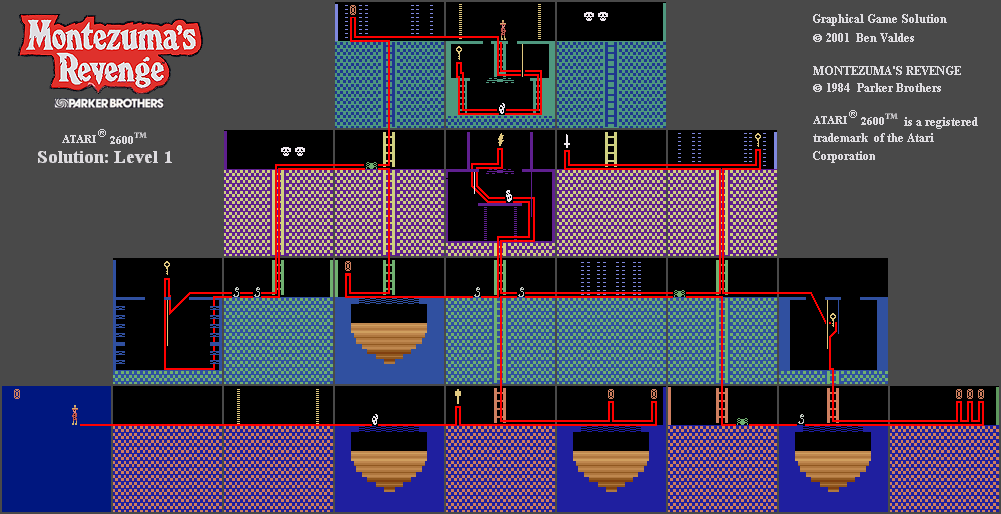
\includegraphics[scale=0.3]{../images/montezuma_map.png}}

  \begin{itemize}
    \item extreme sparse rewards
    \item huge state space
    \item need to return hundrets of steps back
    \item still not solved - without game state save/load
  \end{itemize}

\end{frame}


\begin{frame}{\bf state of the art score}

\begin{columns}
    \column{\dimexpr\paperwidth-10pt}

      source : \url{https://paperswithcode.com/sota/atari-games-on-atari-2600-montezumas-revenge}


      \begin{table}[]
      \begin{tabular}{|l|l|l|}
      \hline
      \textbf{year} & \textbf{name}                                       & \textbf{score} \\ \hline
      2015          & Deep Reinforcement Learning with Double Q-learning  & 0              \\ \hline
      2017          & Curiosity-driven Exploration by Self-supervised Prediction \footnote[1]{https://arxiv.org/abs/1705.05363} & 0       \\ \hline 
      2021          & MuZero                                              & 2500           \\ \hline
      2018          & Count-Based Exploration with Neural Density Models \footnote[2]{https://arxiv.org/abs/1703.01310}  & 3705           \\ \hline
      \textbf{2019} & \textbf{Exploration by Random Network Distillation} \footnote[3]{https://arxiv.org/abs/1810.12894}& \textbf{8152}  \\ \hline
      2021          & GoExplore$^*$ \footnote[4]{https://arxiv.org/abs/2004.12919}                         & 43 000         \\ \hline
      \end{tabular}
      \end{table}

      {\bf * requires environment state saving/loading}

\end{columns}

\end{frame}


\begin{frame}{\bf hard exploration robotics envs}

  \centering{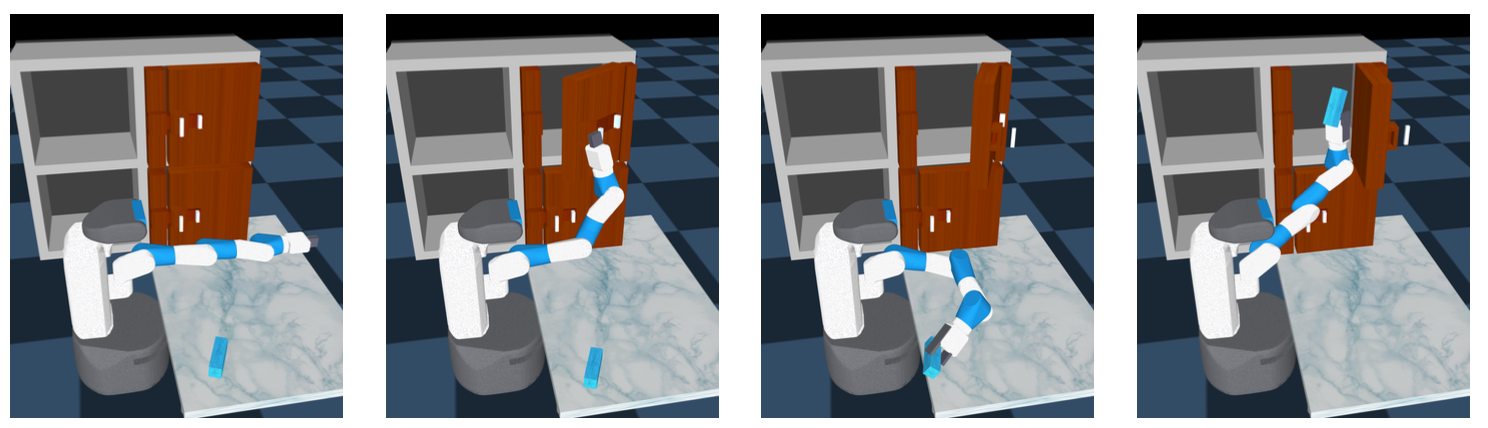
\includegraphics[scale=0.3]{../images/robot_doors.png}}
  \centering{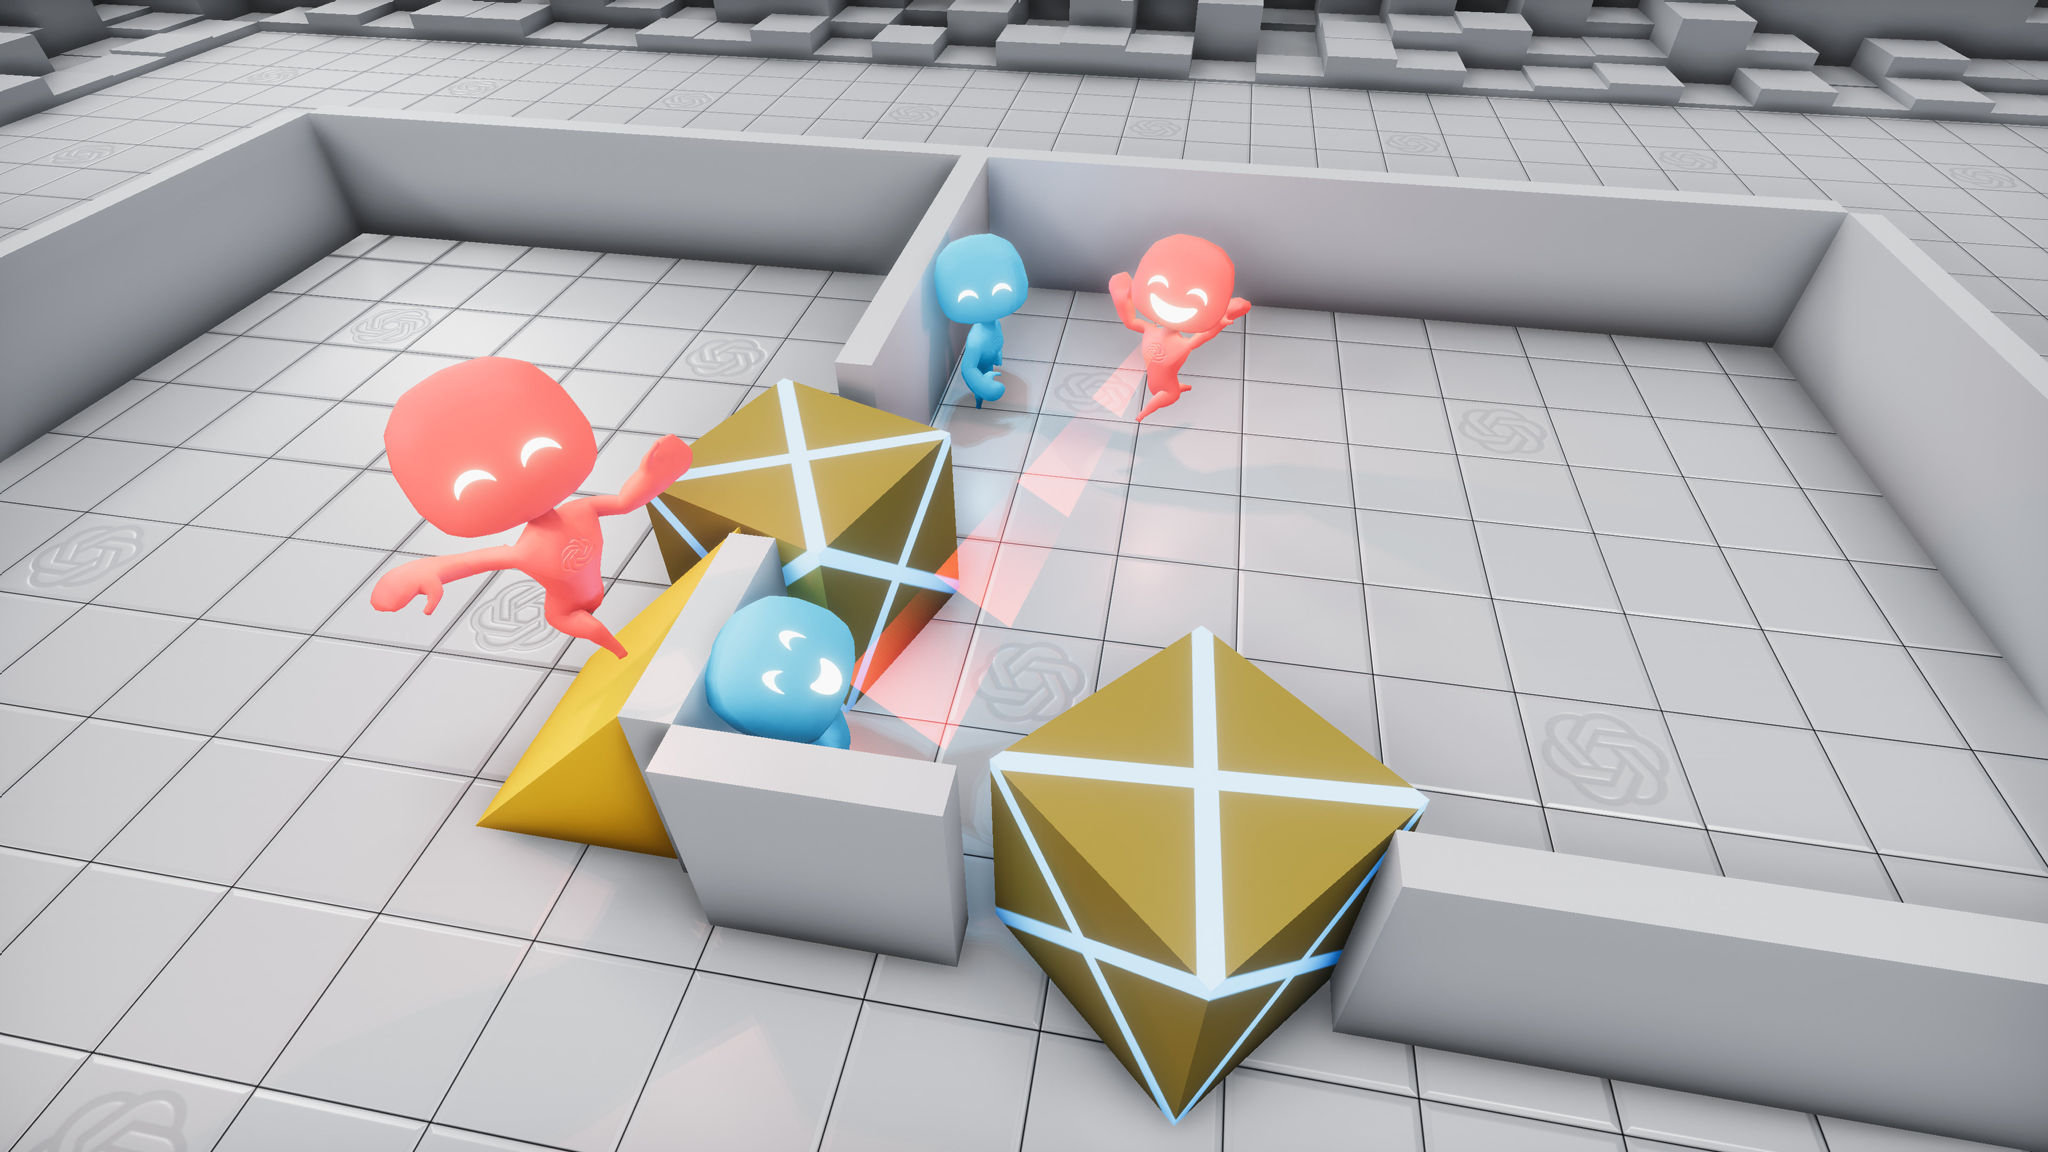
\includegraphics[scale=0.1]{../images/hide_and_seek.jpg}}

\end{frame}

\begin{frame}{\bf wise Wizard's magic staff}

  \begin{columns}

    \begin{column}{0.5\textwidth}
      \begin{itemize}
        \item fully connected nets (robotic envs) {\bf \color{red} train on CPU} - AMD Ryzen
        \item convolutional nets (visual inputs envs) {\bf \color{red} train on GPU}
        \item use fast CPU - envs are slow
        \item 32GB of RAM is enough
        \item for small visual envs (Atari, DOOM, Nec) - GTX1080ti, RTX3060, RTX3080ti ...
      \end{itemize}
    \end{column}

    \begin{column}{0.5\textwidth}
      {\centering 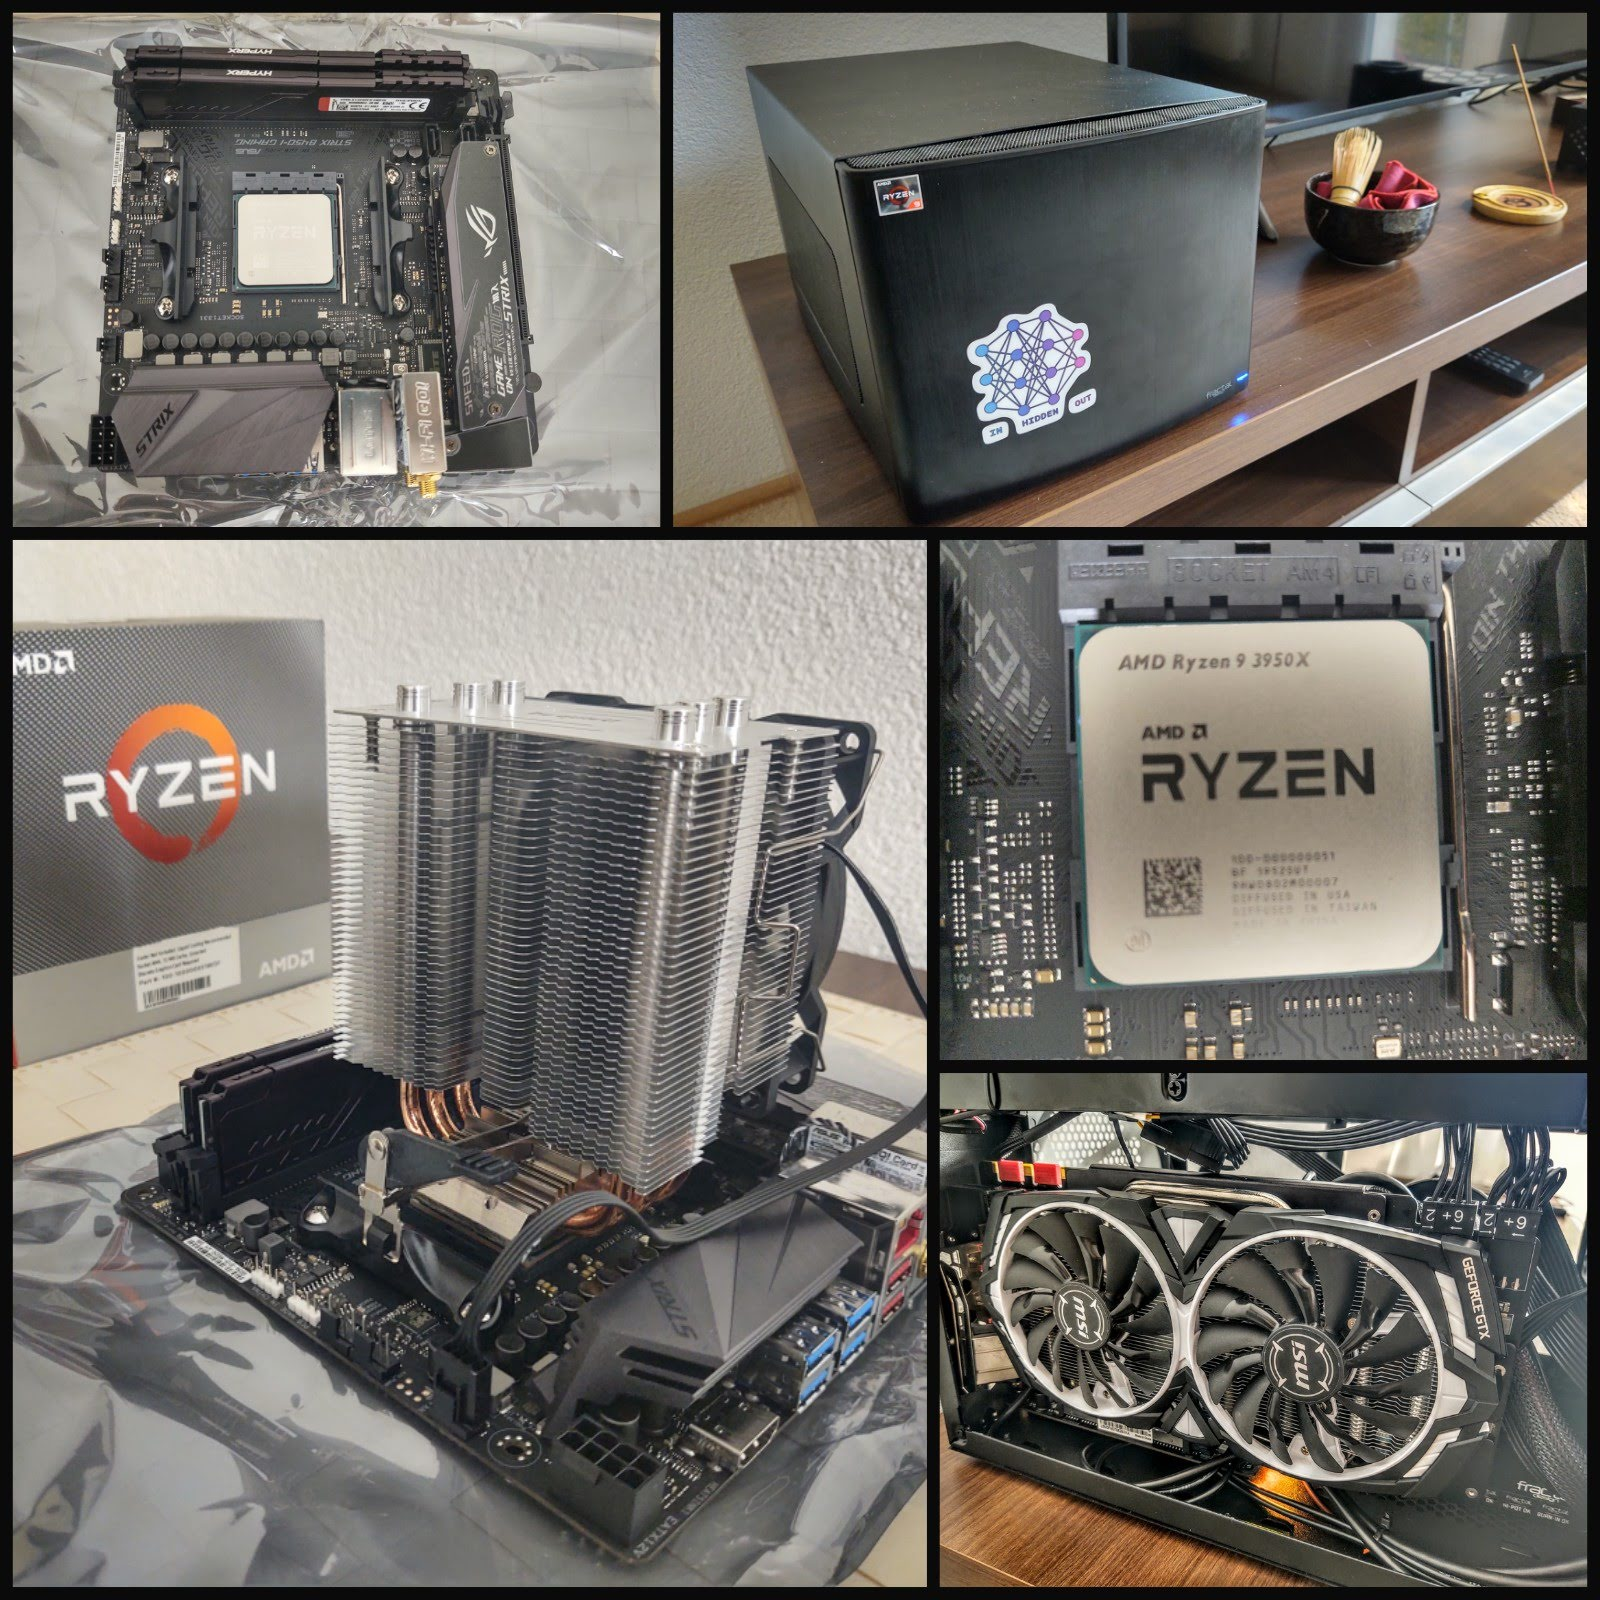
\includegraphics[scale=0.1]{../images/computer.jpg}}
    \end{column}

  \end{columns}


\end{frame}


\begin{frame}{\bf where to start}

\begin{itemize}
  \item simple discrete actions envs : LunarLander, Atari Pong
  \item algorithms : DQN or Dueling DQN
  \item continuous actions envs : LunarLander, Pybullet And + HalfCheetah
  \item algorithms : DDPG
\end{itemize}

{\bf books and blogs}

\begin{itemize}
  \item Maxim Lapan, 2020, Deep Reinforcement Learning Hands-On second edition
  \item Enes Bilgin, 2020, Mastering Reinforcement Learning with Python
  \item Andrej Karpathy, Pong from pixels \url{http://karpathy.github.io/2016/05/31/rl/}
  \item JordiTorresAI, Deep Q-Network, \url{https://towardsdatascience.com/deep-q-network-dqn-i-bce08bdf2af}
\end{itemize}

\end{frame}


\begin{frame}{\bf books to read}

        \begin{itemize}
          \item Maxim Lapan, 2020, Deep Reinforcement Learning Hands-On second edition
          \item Maxim Lapan, 2018, Deep Reinforcement Learning Hands-On
          \item Enes Bilgin, 2020, Mastering Reinforcement Learning with Python
          \item Praveen Palanisamy, 2018, Hands-On Intelligent Agents with OpenAI Gym
          \item Andrea Lonza, 2019, Reinforcement Learning Algorithms with Python
          \item Rajalingappaa Shanmugamani, 2019, Python Reinforcement Learning
          \item Micheal Lanham, 2019, Hands-On Deep Learning for Games
        \end{itemize}

\end{frame}


\begin{frame}{\bf Q\&A}

\centering{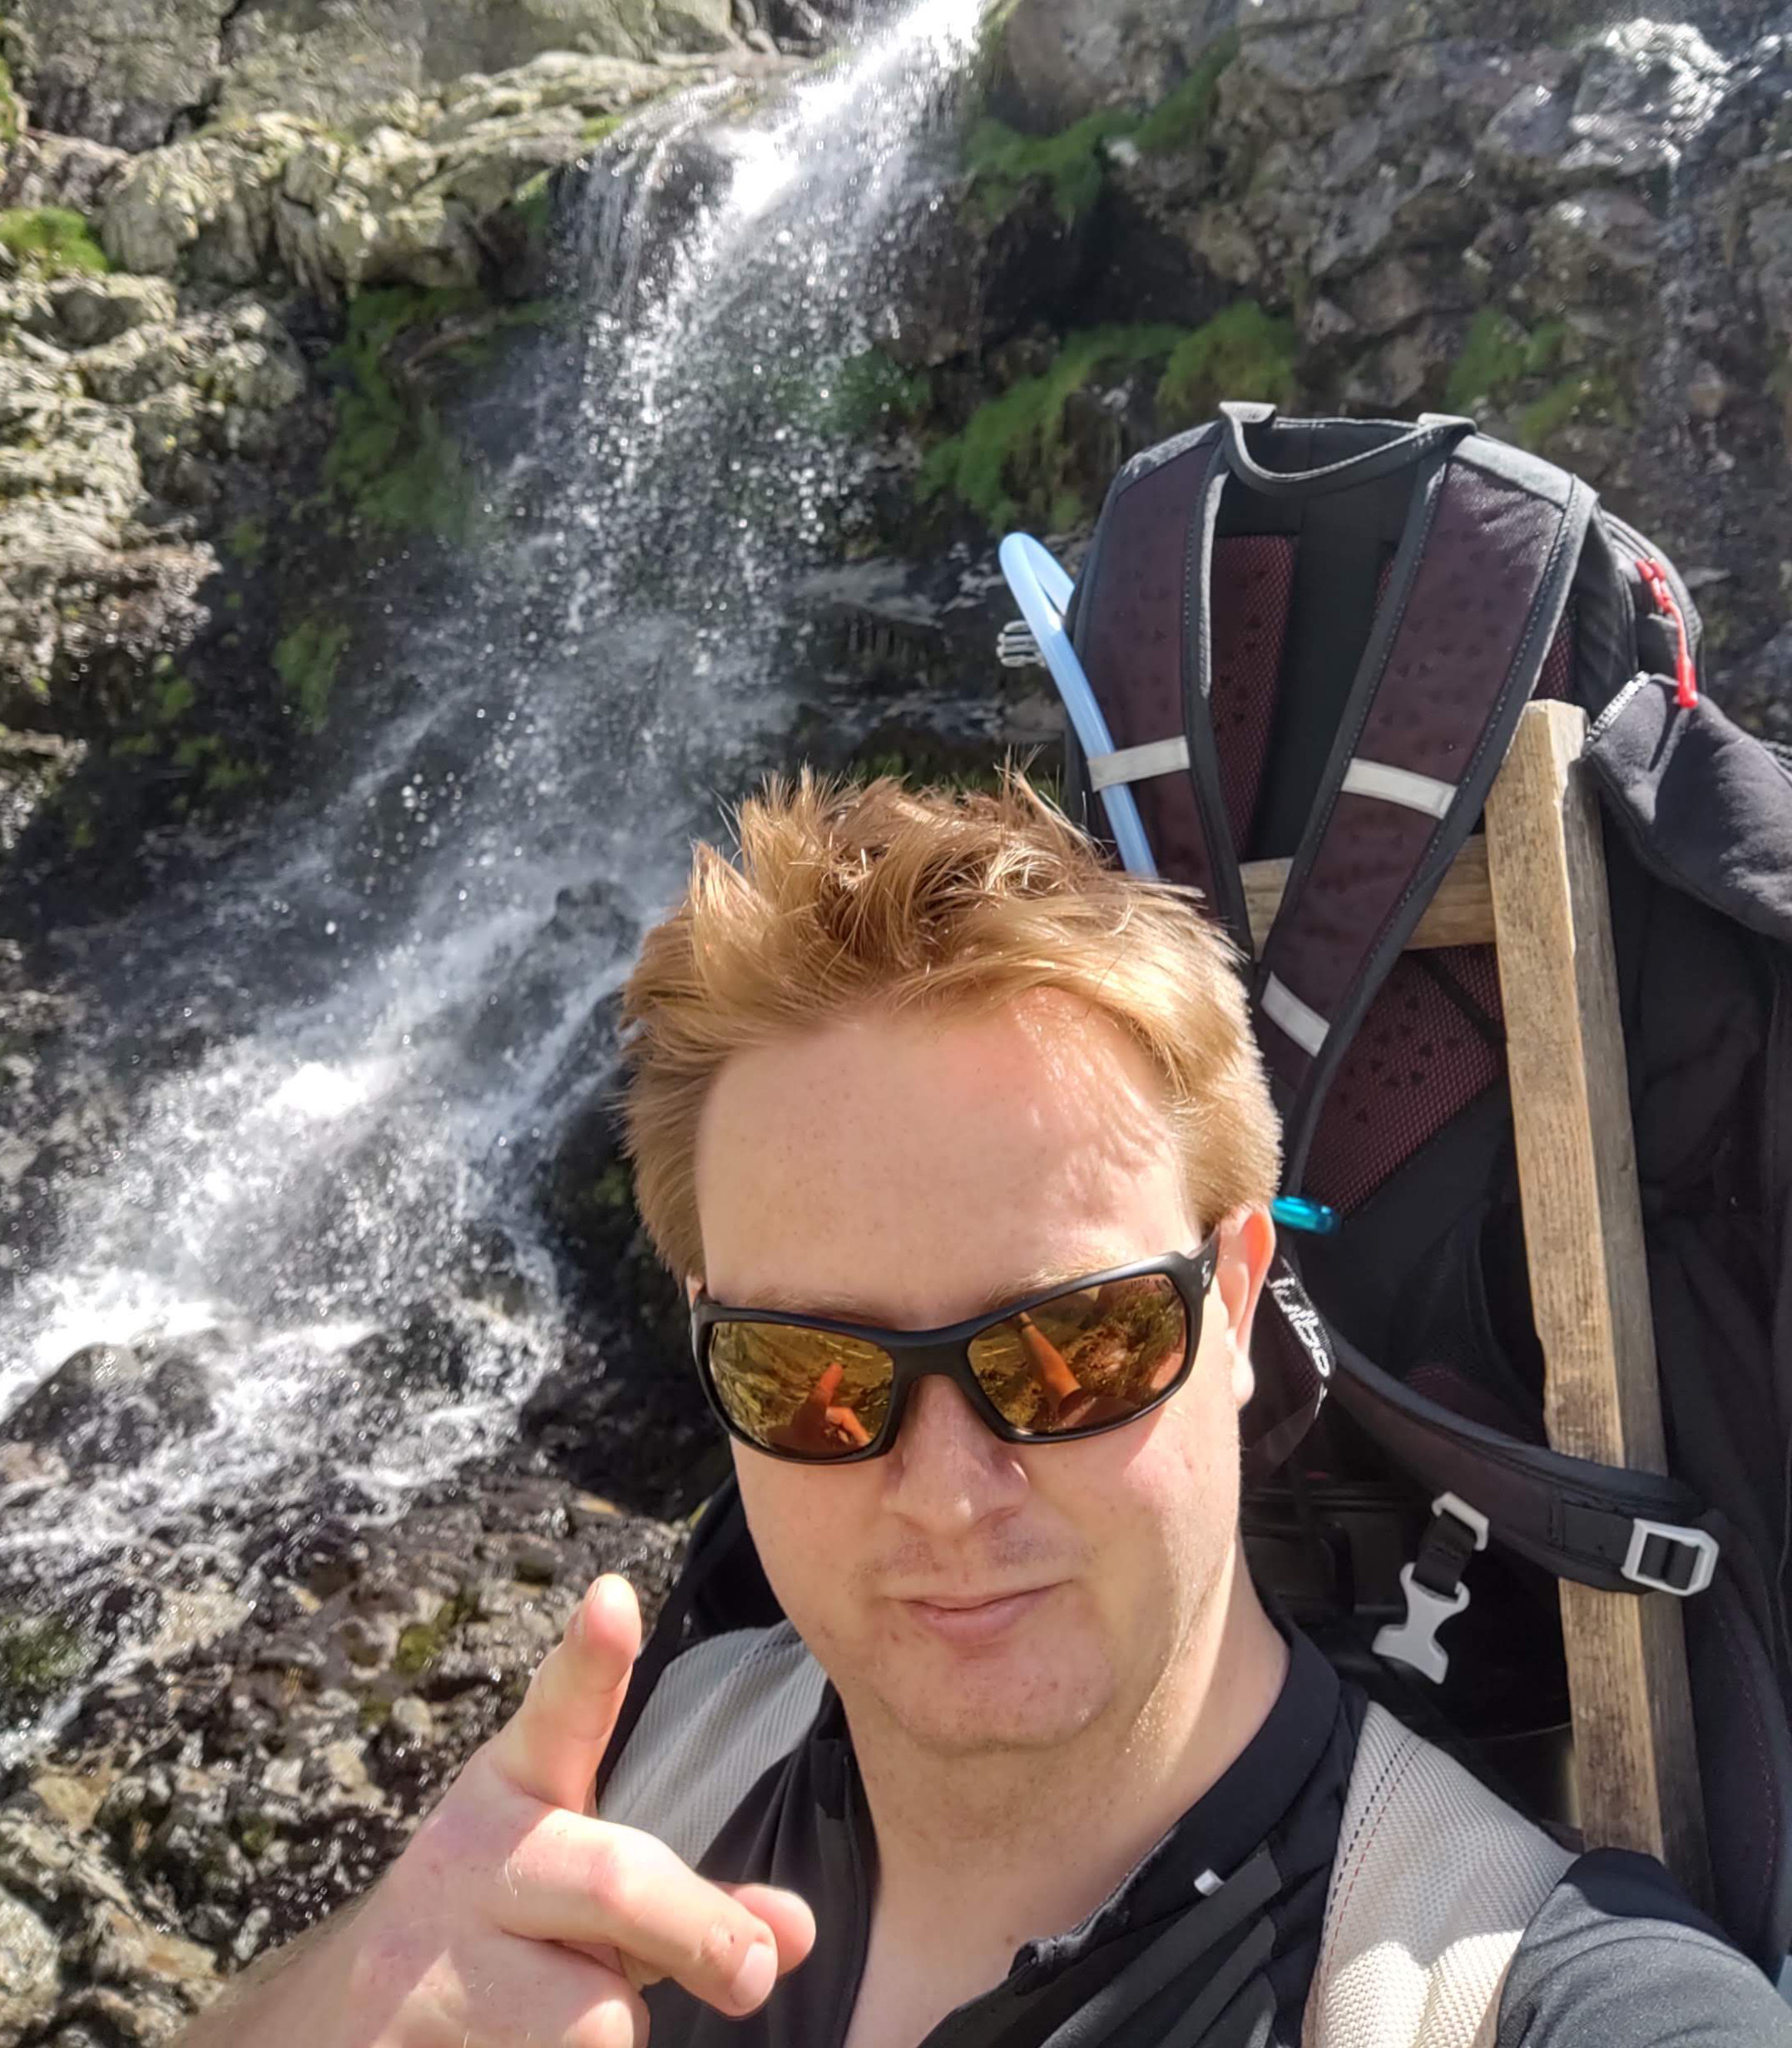
\includegraphics[scale=0.1]{../images/me.jpg}}

\url{michal.nand@gmail.com}

\url{https://github.com/michalnand/imagination_reinforcement_learning}

 \end{frame}


\end{document}
